% Options for packages loaded elsewhere
\PassOptionsToPackage{unicode}{hyperref}
\PassOptionsToPackage{hyphens}{url}
%
\documentclass[
  english,
  man,floatsintext]{apa6}
\usepackage{amsmath,amssymb}
\usepackage{lmodern}
\usepackage{ifxetex,ifluatex}
\ifnum 0\ifxetex 1\fi\ifluatex 1\fi=0 % if pdftex
  \usepackage[T1]{fontenc}
  \usepackage[utf8]{inputenc}
  \usepackage{textcomp} % provide euro and other symbols
\else % if luatex or xetex
  \usepackage{unicode-math}
  \defaultfontfeatures{Scale=MatchLowercase}
  \defaultfontfeatures[\rmfamily]{Ligatures=TeX,Scale=1}
\fi
% Use upquote if available, for straight quotes in verbatim environments
\IfFileExists{upquote.sty}{\usepackage{upquote}}{}
\IfFileExists{microtype.sty}{% use microtype if available
  \usepackage[]{microtype}
  \UseMicrotypeSet[protrusion]{basicmath} % disable protrusion for tt fonts
}{}
\makeatletter
\@ifundefined{KOMAClassName}{% if non-KOMA class
  \IfFileExists{parskip.sty}{%
    \usepackage{parskip}
  }{% else
    \setlength{\parindent}{0pt}
    \setlength{\parskip}{6pt plus 2pt minus 1pt}}
}{% if KOMA class
  \KOMAoptions{parskip=half}}
\makeatother
\usepackage{xcolor}
\IfFileExists{xurl.sty}{\usepackage{xurl}}{} % add URL line breaks if available
\IfFileExists{bookmark.sty}{\usepackage{bookmark}}{\usepackage{hyperref}}
\hypersetup{
  pdftitle={Cognitive Music Listening Space: A Multivariate Approach},
  pdfauthor={Brendon Mizener1, Mathilde Vandenberghe2, Hervé Abdi1, \& Sylvie Chollet2},
  pdflang={en-EN},
  pdfkeywords={Music, Perception, Cognition, Multivariate Analyses},
  hidelinks,
  pdfcreator={LaTeX via pandoc}}
\urlstyle{same} % disable monospaced font for URLs
\usepackage{graphicx}
\makeatletter
\def\maxwidth{\ifdim\Gin@nat@width>\linewidth\linewidth\else\Gin@nat@width\fi}
\def\maxheight{\ifdim\Gin@nat@height>\textheight\textheight\else\Gin@nat@height\fi}
\makeatother
% Scale images if necessary, so that they will not overflow the page
% margins by default, and it is still possible to overwrite the defaults
% using explicit options in \includegraphics[width, height, ...]{}
\setkeys{Gin}{width=\maxwidth,height=\maxheight,keepaspectratio}
% Set default figure placement to htbp
\makeatletter
\def\fps@figure{htbp}
\makeatother
\setlength{\emergencystretch}{3em} % prevent overfull lines
\providecommand{\tightlist}{%
  \setlength{\itemsep}{0pt}\setlength{\parskip}{0pt}}
\setcounter{secnumdepth}{-\maxdimen} % remove section numbering
% Make \paragraph and \subparagraph free-standing
\ifx\paragraph\undefined\else
  \let\oldparagraph\paragraph
  \renewcommand{\paragraph}[1]{\oldparagraph{#1}\mbox{}}
\fi
\ifx\subparagraph\undefined\else
  \let\oldsubparagraph\subparagraph
  \renewcommand{\subparagraph}[1]{\oldsubparagraph{#1}\mbox{}}
\fi
% Manuscript styling
\usepackage{upgreek}
\captionsetup{font=singlespacing,justification=justified}

% Table formatting
\usepackage{longtable}
\usepackage{lscape}
% \usepackage[counterclockwise]{rotating}   % Landscape page setup for large tables
\usepackage{multirow}		% Table styling
\usepackage{tabularx}		% Control Column width
\usepackage[flushleft]{threeparttable}	% Allows for three part tables with a specified notes section
\usepackage{threeparttablex}            % Lets threeparttable work with longtable

% Create new environments so endfloat can handle them
% \newenvironment{ltable}
%   {\begin{landscape}\begin{center}\begin{threeparttable}}
%   {\end{threeparttable}\end{center}\end{landscape}}
\newenvironment{lltable}{\begin{landscape}\begin{center}\begin{ThreePartTable}}{\end{ThreePartTable}\end{center}\end{landscape}}

% Enables adjusting longtable caption width to table width
% Solution found at http://golatex.de/longtable-mit-caption-so-breit-wie-die-tabelle-t15767.html
\makeatletter
\newcommand\LastLTentrywidth{1em}
\newlength\longtablewidth
\setlength{\longtablewidth}{1in}
\newcommand{\getlongtablewidth}{\begingroup \ifcsname LT@\roman{LT@tables}\endcsname \global\longtablewidth=0pt \renewcommand{\LT@entry}[2]{\global\advance\longtablewidth by ##2\relax\gdef\LastLTentrywidth{##2}}\@nameuse{LT@\roman{LT@tables}} \fi \endgroup}

% \setlength{\parindent}{0.5in}
% \setlength{\parskip}{0pt plus 0pt minus 0pt}

% \usepackage{etoolbox}
\makeatletter
\patchcmd{\HyOrg@maketitle}
  {\section{\normalfont\normalsize\abstractname}}
  {\section*{\normalfont\normalsize\abstractname}}
  {}{\typeout{Failed to patch abstract.}}
\patchcmd{\HyOrg@maketitle}
  {\section{\protect\normalfont{\@title}}}
  {\section*{\protect\normalfont{\@title}}}
  {}{\typeout{Failed to patch title.}}
\makeatother
\shorttitle{Music Descriptor Space}
\keywords{Music, Perception, Cognition, Multivariate Analyses\newline\indent Word count: 5631}
\usepackage{csquotes}
\usepackage{caption}
\usepackage{subcaption}
\usepackage{wrapfig}
\ifxetex
  % Load polyglossia as late as possible: uses bidi with RTL langages (e.g. Hebrew, Arabic)
  \usepackage{polyglossia}
  \setmainlanguage[]{english}
\else
  \usepackage[main=english]{babel}
% get rid of language-specific shorthands (see #6817):
\let\LanguageShortHands\languageshorthands
\def\languageshorthands#1{}
\fi
\ifluatex
  \usepackage{selnolig}  % disable illegal ligatures
\fi
\newlength{\cslhangindent}
\setlength{\cslhangindent}{1.5em}
\newlength{\csllabelwidth}
\setlength{\csllabelwidth}{3em}
\newenvironment{CSLReferences}[2] % #1 hanging-ident, #2 entry spacing
 {% don't indent paragraphs
  \setlength{\parindent}{0pt}
  % turn on hanging indent if param 1 is 1
  \ifodd #1 \everypar{\setlength{\hangindent}{\cslhangindent}}\ignorespaces\fi
  % set entry spacing
  \ifnum #2 > 0
  \setlength{\parskip}{#2\baselineskip}
  \fi
 }%
 {}
\usepackage{calc}
\newcommand{\CSLBlock}[1]{#1\hfill\break}
\newcommand{\CSLLeftMargin}[1]{\parbox[t]{\csllabelwidth}{#1}}
\newcommand{\CSLRightInline}[1]{\parbox[t]{\linewidth - \csllabelwidth}{#1}\break}
\newcommand{\CSLIndent}[1]{\hspace{\cslhangindent}#1}

\title{Cognitive Music Listening Space: A Multivariate Approach}
\author{Brendon Mizener\textsuperscript{1}, Mathilde Vandenberghe\textsuperscript{2}, Hervé Abdi\textsuperscript{1}, \& Sylvie Chollet\textsuperscript{2}}
\date{}


\authornote{

Add complete departmental affiliations for each author here. Each new line herein must be indented, like this line.

Enter author note here.

The authors made the following contributions. Brendon Mizener: Stimuli creation, Survey design \& creation, Data collection \& processing, Statistical analyses, Writing - Original draft preparation; Mathilde Vandenberghe: Original concept, Survey design \& creation; Hervé Abdi: Writing - Review \& Editing, Statistical guidance; Sylvie Chollet: Original concept.

Correspondence concerning this article should be addressed to Brendon Mizener, 800 W. Campbell Rd., Richardson Tex. E-mail: \href{mailto:bmizener@utdallas.edu}{\nolinkurl{bmizener@utdallas.edu}}

}

\affiliation{\vspace{0.5cm}\textsuperscript{1} University of Texas at Dallas\\\textsuperscript{2} Junia, Univ. Artois, Université de Liège, Univ. Littoral Côte d'Opale, UMRT 1158 BioEcoAgro, F-62000 Arras, France}

\abstract{
French and American participants listened to new music stimuli and evaluated the stimuli using either adjectives or quantitative musical dimensions. Results were analyzed using Correspondence Analysis (CA), Hierarchical Cluster Analysis (HCA), Multiple Factor Analysis (MFA), and Partial Least Squares Correlation (PLSC). French and American listeners differed when they described the musical stimuli using adjectives, but not when using the quantitative dimensions. The present work serves as a case study in research methodology that allows for a balance between relaxing experimental control and maintaining statistical rigor.
}



\begin{document}
\maketitle

We have a data collection problem: World events over the last year have shown that we need to be able to collect good data outside of the lab. In the lab, because we control error sources, we measure, on relatively small sets of observations, a few well-defined, quantitative variables, analyzed using standard techniques such as analysis of variance (ANOVA). But, with the labs closed (remember COVID?), how can we collect good data? Away from the controlled environment of the lab, quantitative variables are hard to measure, but we can collect, on large sets of observations, qualitative variables that can only be analyzed by newer multivariate techniques. In the present paper, we present a case study illustrating this tradeoff.

In 2004, Zampini \& Spence demonstrated that something as simple as the sound of the crunch could influence the taste of a potato chip (Zampini \& Spence, 2004). What about a signal as complex as a string quartet? The present study was designed to quantify a music listening ``space'' that captures objective stimulus and cognitive dimensions to use in future studies investigating cross-modal sensory mapping between beer drinking and music listening.

For the present study, we have defined stimulus dimensions as quantitative musical qualities, such as tempo, range, and meter and cognitive dimensions as qualitative descriptions of music, such as ``Dark,'' ``Warm,'' and ``Round.'' These cognitive/qualitative dimensions are similar to the commonly investigated affective or emotional dimensions, but do not specifically assess affective quality. We designed three experiments to quantify individual and combined spaces for these concepts, using separate surveys. The first experiment included highly trained musicians and featured a multiple-choice survey about the stimulus dimensions; the second included participants with any level of music training performing a check-all-that-apply task (CATA, Katz \& Braly, 1933; Meyners \& Castura, 2014; Coombs et al., 1956); the third experiment incorporated both surveys in a single analysis.

To analyze our data, we selected a set of multivariate analyses that allowed us to visualize answers to each of our questions. Each of these multivariate analyses serve to reduce the dimensionality of a data set by computing new variables, or dimensions, that represent the important information in the table, and factor scores, which can be plotted as points in the space defined by these new variables. The space revealed by an analysis can show similarity among variables or observations, and can be interpreted as conceptual or mental spaces (Abdi \& Williams, 2010).

The mental spaces revealed by the individual surveys were calculated and visualized using Correspondence Analysis (CA), a method similar to Principal Components Analysis (PCA) that analyzes qualitative data. We used Multidimensional Scaling (MDS), a distance analysis, to visualize the differences between participants and participant groups. To find parallels between the surveys, we used Partial Least Squares Correlation (PLSC), a method that analyzes two data tables with different sets of variables measured on the same observations. We used a Multiple Factor Analysis (MFA) to evaluate how French and American participants' responses differed. Each of these analyses provide different visualizations and interpretations of the data, which are discussed in more detail below.

\hypertarget{music-perception}{%
\subsection{Music Perception}\label{music-perception}}

Quantifying music perception is an interesting test case for this kind of data gathering and analytical paradigm. Most music or auditory perception studies have the inherent confound that small changes can affect listeners' perception, especially when the study involves timing, tuning, or sound localization. However, the experimental controls may be loosened slightly when investigating holistic music listening, because no single musical element is more important than the whole.

Quantitative and qualitative elements of music are theoretically distinct but practically inseparable (Bruner II, 1990). Listeners respond affectively to technical aspects of music using schemata informed by their individual musical experiences and personality traits (Kopacz, 2005), and composers use various musical and compositional techniques to convey the emotions they want to express (Battcock \& Schutz, 2019; Bruner II, 1990). However, quantifying the perceptual interactions between more than one or two musical qualities is a challenge. One reason is that models such as ANOVA and its variations are limited by how many variables a researcher can include while remaining coherent. Another is that asking participants to respond to multiple aspects of a stimulus taxes participants' perceptual capacity and is thus difficult to measure (W. F. Thompson, 1994).

One specific area that has attempted to capture a greater dimensionality is music emotion research. This is a well trod domain---see, for example Juslin and Sloboda (2010)---and the application of multivariate analyses to these questions is similarly well established. Early studies, including Gray and Wheeler (1967), Wedin (1969), and Wedin (1972) used MDS to capture the affective space of various musical stimuli. MDS continues to be used commonly in more modern studies (Bigand et al., 2005; Madsen, 1997; Rodà et al., 2014), with a narrow focus on valence and arousal, which were first proposed to be the most salient dimensions of perception by Osgood and Suci (1955).

A few studies have specifically investigated dimensions beyond those first two (for example Rodà et al., 2014), and there are conflicting hypotheses about whether the valence-arousal plane or a different model of emotion perception represents the fundamental space around music emotion perception (Cowen et al., 2020; Juslin \& Västfjäll, 2008). However, an important distinction between the present study and work in music emotion perception is that the adjectives we chose were informed by music composition and performance, rather than emotion (Wallmark, 2019).

With regard to musical expertise, there are many studies that evaluate the differences between trained and untrained listeners, but the verdict as to whether trained musicians are better listeners is still out, partially due to the fact that there is little standardization in how much training is required for a participant to be ``highly trained'' (Bigand \& Poulin-Charronnat, 2006). There are, however, reported benefits with regard to sensitivity to the emotional content in music (Ladinig \& Schellenberg, 2012) and familiarity with tonal systems (Bartlett \& Dowling, 1980; Dowling, 1978). Recent works suggest that these benefits may be limited to specific technical aspects, and depend on the extent of training (Raman \& Dowling 2017). Although we do not specifically evaluate the differences between trained and untrained listeners in the present study, we included highly trained musicians because they are sensitive to these technical aspects of music and will be able to accurately quantify the stimuli. Additionally, some of the response options to questions on the survey for Experiment 1 would only be familiar to participants with significant music training.

\hypertarget{intercultural-music-perception}{%
\subsubsection{Intercultural music perception}\label{intercultural-music-perception}}

There are a few common goals in intercultural studies of music perception. Some quantify the shared emotional experience between musical cultures (Balkwill et al., 2004; Balkwill \& Thompson, 1999; Cowen et al., 2020; Darrow et al., 1987; Fritz et al., 2009; Gregory \& Varney, 1996), and some ask participants to identify technical aspects of music from other cultures (Raman \& Dowling, 2016, 2017). There are fewer studies that include the semantics of language in their evaluation of music perception (Zacharakis et al., 2014, 2015), which makes this a prime area for research.

The research program presented in Zacharakis et al. (2014) and Zacharakis et al. (2015) deals specifically with timbre perception, and their use of adjectives is similar to the way adjectives are used in the present study. In Zacharakis et al.~(2014, 2015), Greek and English participants described timbre with adjectives from their native languages. These studies found that while there are some differences, overall, participants' descriptions of timbre do not differ much between languages (Zacharakis et al., 2014, 2015).

\hypertarget{present-questions-methods-of-analysis}{%
\subsection{Present questions \& methods of analysis}\label{present-questions-methods-of-analysis}}

The primary question addressed in this study is: Can we quantify a cognitive space around music listening defined by both stimulus and cognitive dimensions of music. Secondary questions include whether French and American participants describe music differently, and whether those differences may arise from cultural differences in music listening or preferences or are purely semantic. To answer these questions, we employed a set of multivariate analyses that each offered a different perspective on the results of each experiment. We felt it may be useful to provide a quick overview of the data collection and analytical techniques for readers who may be unfamiliar.

\hypertarget{check-all-that-apply-cata}{%
\subsubsection{Check-all-that-apply (CATA)}\label{check-all-that-apply-cata}}

The CATA technique---a method widely used in sensory evaluation---measures how participants describe a set of stimuli (Coombs et al., 1956; Katz \& Braly, 1933; Meyners \& Castura, 2014; Valentin et al., 2012). In a CATA task, stimuli are presented one at a time, and for each stimulus, participants are shown a list of descriptors and are asked to select the descriptors that describe the presented stimulus (Meyners \& Castura, 2014). CATA easily assesses questions with multiple ``correct'' responses (Coombs et al., 1956), and places little cognitive demand on participants because they do not have to generate responses (Ares et al., 2010).\\
CATA data are analyzed by 1) computing a pseudo contingency table that records the number of times descriptors were associated with stimuli and 2) analyzing this data table with Corresponence Analysis (CA) in order to visualize the patters of association between a) stimuli, b) descriptors, and c) stimuli and descriptors.

\hypertarget{correspondence-analysis}{%
\subsubsection{Correspondence Analysis}\label{correspondence-analysis}}

The primary analysis used on the stimulus response data collected in the surveys is Correspondence Analysis (CA) (Benzécri, 1973; Escofier-Cordier, 1965; Greenacre, 1984). CA analyzes a contingency table, or any data structured similarly, and calculates the relationships between rows (observations) and columns (variables); in our case, musical excerpts and descriptors. The nature of the CA allows for observations and variables to be visualized in the same space.

\hypertarget{hierarchical-cluster-analysis}{%
\subsubsection{Hierarchical Cluster Analysis}\label{hierarchical-cluster-analysis}}

Hierarchical Cluster Analysis (HCA) (Pielou, 1984) is a way of identifying groups, or clusters, of observations from the rows of a distance matrix, that are displayed using trees to visualize that distance. This technique was used in the present study to determine whether there were any clusters of excerpts or adjectives that arose during participant ratings. These clusters were used as design or grouping variables and to select colors for visualizations.

\hypertarget{multidimensional-scaling}{%
\subsubsection{Multidimensional Scaling}\label{multidimensional-scaling}}

Multidimensional Scaling (MDS) (Borg \& Groenen, 2005)---a technique commonly used in music perception studies (Bigand et al., 2005; Madsen, 1997; Rodà et al., 2014; Wedin, 1969, 1972) analyzes a distance matrix computed between observations and visualizes them, positioning these observations on a map such that the distance between observations on the map best approximates their distance in the data table. In the present study, this technique is used as an omnibus test to evaluate similarity between groups of participants.

\hypertarget{multiple-factor-analysis}{%
\subsubsection{Multiple Factor Analysis}\label{multiple-factor-analysis}}

Multiple Factor Analysis (MFA) (Abdi et al., 2013; Escofier \& Pagès, 1994) is an extension of PCA that analyzes and visualizes multiple tables or blocks of variables that each describe the same observations. MFA computes \emph{compromise} and \emph{partial factor scores}, where the \emph{compromise} is the average of (or compromise between) the normalized factor scores from each block, and the \emph{partial factor scores} are the factor scores of each individual block. Plotting these factor scores allows for the comparison of observations (rows), and, for each observation, the relationships between the blocks of variables that contributed to that observation. Practically speaking, the most basic difference between MFA and PLSC is that PLSC extracts commonalities between two data tables, whereas MFA extracts similarities and differences between two or more data tables. In the present study, this technique was used to evaluate differences between French and American participants in how they described specific excerpts and used specific adjectives.

\hypertarget{partial-least-squares-correlation}{%
\subsubsection{Partial Least Squares Correlation}\label{partial-least-squares-correlation}}

Partial Least Squares Correlation (PLSC) (Abdi \& Williams, 2013; Tucker, 1958) analyzes two data tables that describe the same set of observations (rows) with two different sets of variables (columns). To extract the common information between the two data tables, PLSC separately combines the variables from each data table to create new variables---similar to factor scores---called latent variables, that have the largest covariance. This method is commonly used in neuroimaging studies to extract the common information between imaging and behavioral data (Krishnan et al., 2011). It was used in the present study to evaluate the similarities in how participants in either survey rated the excerpts.

\hypertarget{bootstrapping}{%
\subsubsection{Bootstrapping}\label{bootstrapping}}

We use bootstrapping (Hesterberg, 2011) to evaluate group differences because the methods outlined above are not inferential methods, and do not inherently allow for hypothesis testing. Bootstrapping evaluates the stability of the result of an experiment. This is displayed in the form of confidence intervals, as ellipses, in the plots below, computed from resampling the original observations (Hesterberg, 2011).

\hypertarget{experiment-1-musical-qualities-survey}{%
\section{Experiment 1: Musical Qualities Survey}\label{experiment-1-musical-qualities-survey}}

\hypertarget{methods}{%
\subsection{Methods}\label{methods}}

\hypertarget{participants}{%
\subsubsection{Participants}\label{participants}}

For the first experiment, we recruited highly trained musicians with a minimum of 10 years of formal music training to evaluate the stimulus dimensions or musical qualities of the stimuli, and to ascertain whether the stimuli truly reflected the composer's intent of varying on a wide range of musical dimensions (Raman \& Dowling, 2017). Participants in the United States and in France were recruited by word of mouth and social media. There were a total of 84 responses to the survey, of which 57 were removed for not completing the survey, leaving a total of 27 (N\(\mathrm{_{France}}\) = 9, N\(\mathrm{_{USA}}\) = 18) for the analysis. All recruitment measures were approved by the UT Dallas IRB.

\hypertarget{stimuli}{%
\subsubsection{Stimuli}\label{stimuli}}

All stimuli were new, original excerpts, in various Western styles, composed using Finale composition software (Finale v25, MakeMusic, Inc.) by the first author specifically for this study (scores and audio files available upon request). Each stimulus was a wav file generated using the Finale human playback engine, approximately 30 s in length (range: 27-40 s, \emph{M} = 32.4 s). The stimuli were all string quartets, in order to control for effects of timbre and otherwise vary on a number of musical qualities, specifically Harmony, Tempo, Meter, Density, and Genre. The stimuli are numbered by the order in which they were composed and thus do not reflect any specific grouping. Participants were not made aware of excerpt numbers during the course of the experiment.

\hypertarget{survey}{%
\subsubsection{Survey}\label{survey}}

American and French participants received links to surveys presented in English and French, respectively, both presented via Qualtrics. Participants were instructed to listen to the listen to the excerpts presented in the survey using headphones or in a quiet listening environment, but that was not controlled, nor was it assessed as part of the survey. After standard informed consent procedures, participants listened to 15 of the 30 excerpts, presented one at time in a random order, and answered ten questions per excerpt, one for each of the musical qualities being assessed. The musical qualities assessed and the levels associated with each are indicated in Table \ref{tab:qualitiestable}. Of these dimensions being assessed, all were multiple choice, allowing for a single response, except for meter, contour, and articulation, which were check-all-that-apply. See supplementary materials for the French translations of this table. Upon completion of the experimental task, participants were asked to provide demographic data, including age, gender identity, nationality, occupation, and musical experience.

\begin{lltable}
\begin{scriptsize}
\begin{longtable}{p{0.2\textwidth}p{0.2\textwidth}p{0.2\textwidth}p{0.2\textwidth}p{0.2\textwidth}p{0.2\textwidth}}\noalign{\getlongtablewidth\global\LTcapwidth=\longtablewidth}
\caption{\label{tab:qualitiestable}Musical Qualities and the provided survey response options.}\\
\toprule[.8pt]
 \multicolumn{1}{c}{Harmonic Material} & \multicolumn{1}{c}{Tempo} & \multicolumn{1}{c}{Meter} & \multicolumn{1}{c}{Density} & \multicolumn{1}{c}{Genre} & \multicolumn{1}{c}{Articulation}\\
 \midrule
      Diatonic: Major & Very slow & Simple Duple & Very sparse & Baroque & Staccato \\
      Diatonic: Minor & Slow & Simple Triple & Moderately sparse & Classical & Marcato \\
      Blues & Moderately Slow & Simple Quadruple  & More sparse than dense & Romantic & Legato\\
      Chromatic & Moderate & Compound Duple & More dense than sparse & Impressionist & Tenuto\\
      Whole tone & Moderately Fast & Compound Triple & Moderately Dense & Modern & Other \\       
      Modal  & Fast & Compound Quadruple & Very Dense & Jazz/Blues & \\
      Quintal/Quartal  & Very Fast & Complex & & Contemporary & \\
      Ambiguous  & & & & Other & \\
      Other  & & & & & \\
\bottomrule\addlinespace[.5em]
 & \multicolumn{1}{c}{Contour} & \multicolumn{1}{c}{Motion} & \multicolumn{1}{c}{Range} & \multicolumn{1}{c}{Dynamics} & \\
 \cmidrule[.5pt]{2-5}
  & Ascending & Conjunct & Narrow & Soft & \\
  & Descending & Disjunct & Moderate & Moderate  & \\
  & Arch & \multirow{2}{0.2\textwidth}{Combination of conjunct and disjunct} & Wide & Loud  & \\
  & Undulating &  & Very Wide & \multirow{2}{0.2\textwidth}{Varied: gradual crescendo} &\\
  & Pendulum & \multirow{2}{0.2\textwidth}{I do not think this excerpt has a melody} & \multirow{2}{0.2\textwidth}{I do not think this excerpt has a melody} &  &\\
  & Terrace & & & \multirow{2}{0.2\textwidth}{Varied: gradual decrescendo} & \\
  & \multirow{2}{0.2\textwidth}{I do not think this excerpt has a melody} & Other & & &\\
  & & & & \multirow{2}{0.2\textwidth}{Some of each, soft and loud}   & \\
  & Other & & & & \\
  & & & & Other & \\
  
\cmidrule[.75pt]{2-5}
\end{longtable}
\end{scriptsize}
\end{lltable}

\hypertarget{data-processing}{%
\subsubsection{Data Processing}\label{data-processing}}

To process the data, survey responses were converted into a ``brick'' of data, with the excerpts on the rows, the qualities on the columns, and the participants on the pages. For the current experiment, one quality is one variable, and we refer to the response options as levels of that variable. On any page, at the intersection of any row and column was a one or a zero, with a one indicating that this participant had selected this level of this quality (column) to describe this excerpt (row). The responses in the French ``brick'' were all translated into English, and then the bricks from both nationalities were summed together across pages to obtain a single pseudo-contingency table\footnote{Whereas, in a contingency table, there is one and only one ``1'' in each row---a pattern indicating that each observation (row) is associated with a single variable (column)---by contrast, in a pseudo-contingency table, there are as many ones as variables the participant decided were associated with that observation.} in which the intersection of a row and a column was the total number participants who selected a level of a musical quality to describe an excerpt. Levels for which the column sum was equal to one were considered as outliers and removed from the data. Figure \ref{fig:dataflow} shows the data manipulation process graphically.

\begin{figure}   
  \centering  
  \caption{Survey data processing flowchart. In the top table, participants are in rows and excerpts are in blocks of columns. Purple cells indicate that participants were presented with and responded to an excerpt, gray cells indicate that participants were not presented with an excerpt.}
    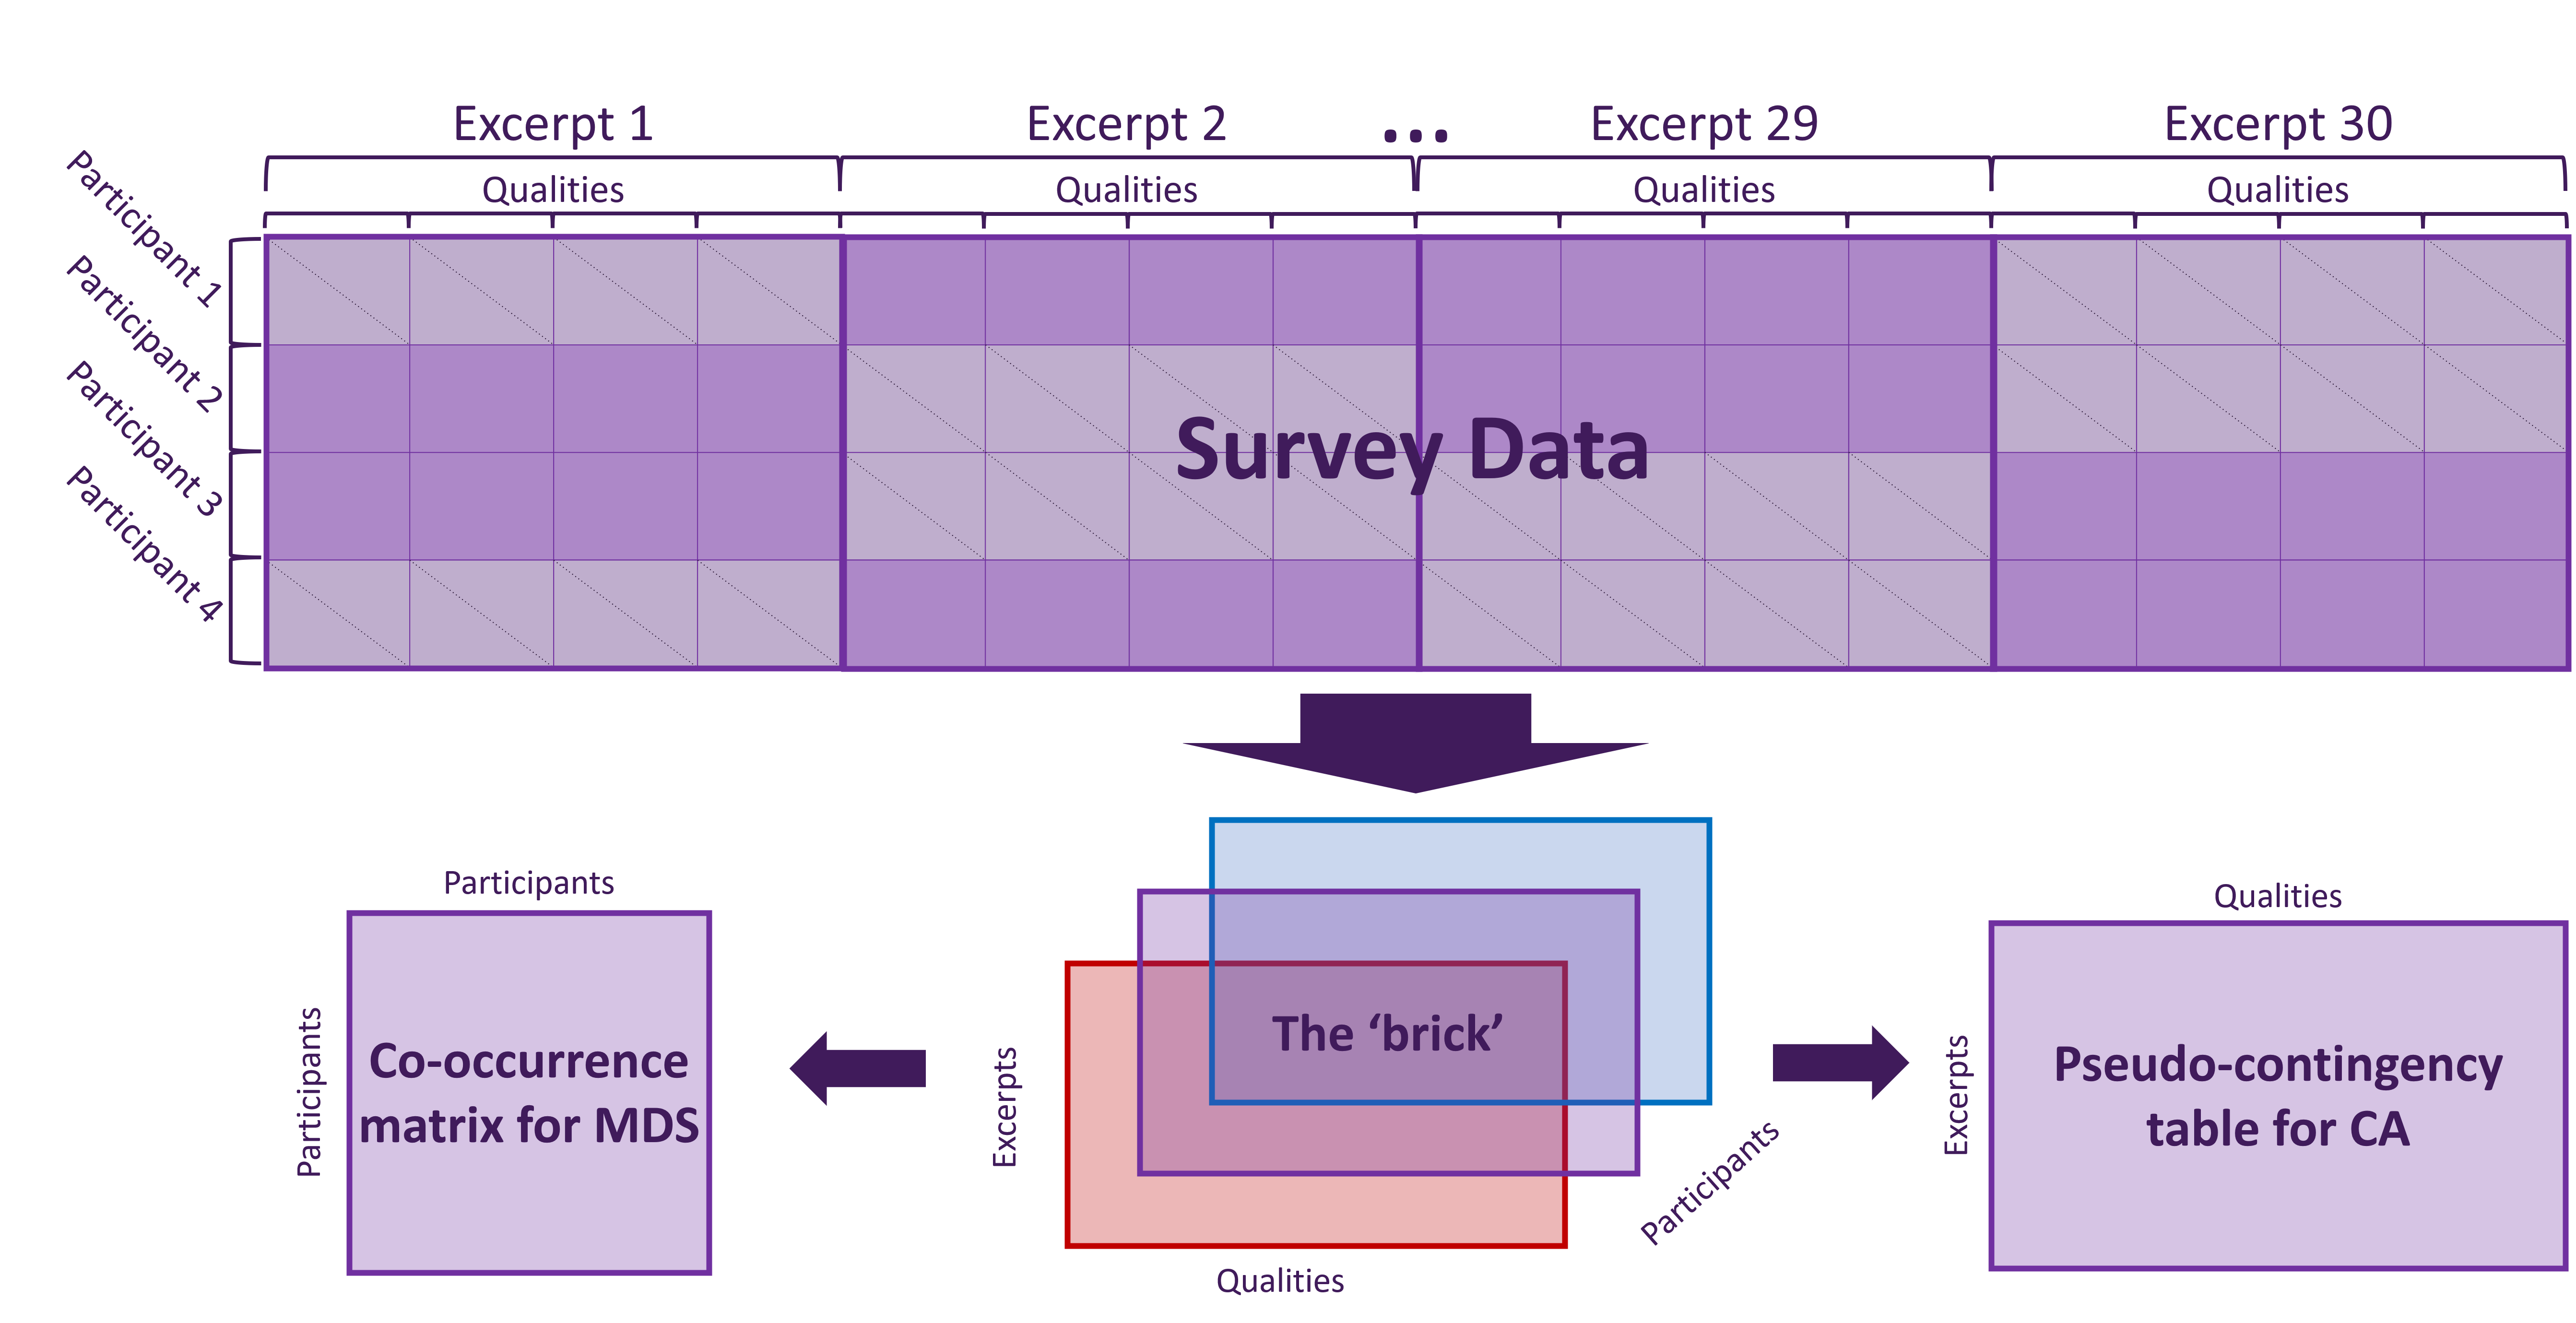
\includegraphics[width=1\columnwidth]{./Music-Descriptor-Space_files/figure-latex/dataflow.png}
  \label{fig:dataflow}
  \caption*{\footnotesize }
\end{figure}

After removing these columns, preliminary visualizations revealed a few variables that required recoding because they were having an outsized effect on the analysis. For the ``Meter,'' variable, there were initially seven levels: ``Simple Duple,'' ``Simple Triple,'' ``Simple Quadruple,'' ``Compound Duple,'' ``Compound Triple,'' ``Compound Quadruple,'' and ``Complex,'' but some participants misunderstood this question and selected multiple options for each level of ``Duple,'' ``Triple'' or ``Quadruple.'' These responses were recoded, removing ``Simple,'' ``Compound'' and ``Complex,'' (there were no excerpts with complex meter), and collapsed, so that each excerpt had only one meter response per participant, ``Duple,'' ``Triple,'' or ``Quadruple.''

There were multiple qualities for which a possible response was ``I do not think this excerpt has a melody,'' and this pattern created a problem in which multiple columns represented the same response, which had a similar effect to the one caused by the ``Meter'' variable before it was recoded. To avoid this problem, these responses were also recoded. A new variable, ``Melody,'' was created, with two levels/columns, yes and no, and if participants responded ``I do not think this excerpt has a melody'' to any of the Contour, Motion, or Range variables, a one was counted in the ``No'' column for that participant and that excerpt. The other levels for each of these three variables were then recoded so that each other column for that variable in that row had the value of one divided by the number of options for that variable---a procedure called barycentric recoding. If the participant responded with ``I do not think this excerpt has a melody'' for some but not all three of those variables, a one was still counted in the ``no melody'' column, but only the variables for which ``I do not think\ldots{}'' was selected were recoded using barycentric recoding. For all excerpts and participants for which ``I do not think\ldots{}'' was never selected, a one was added to the ``Yes'' column for the melody variable. Once the data were recoded, the brick was once again summed across pages to obtain the data table that would be used for subsequent analyses.

\hypertarget{analysis}{%
\subsubsection{Analysis}\label{analysis}}

To analyze the similarity structure between participants, we computed a co-occurrence matrix from the brick with participants on the rows and columns, such that the intersection of a row and column represented the number of common choices between participants. This was then analyzed using MDS.

To analyze the excerpts and musical qualities and obtain the music quality space, we performed a CA on the contingency table. To identify potential clusters among the excerpts, we ran an HCA on the row factor scores obtained from the CA.

\hypertarget{results}{%
\subsection{Results}\label{results}}

\hypertarget{participants-1}{%
\subsubsection{Participants}\label{participants-1}}

The MDS performed on the co-occurrence matrix of participants was intended to identify potential clusters of participants. Visual examination of the results did not reveal any clusters---a pattern suggesting that the participants constituted a homogeneous group. To further assess this conclusion, we also computed average factor scores by nationality and gender identity and bootstrap-derived confidence intervals around these averages and did not find any significant differences. See supplementary materials for plots illustrating this.

\begin{wrapfigure}{h}{.4\textwidth}  
  \begin{center}
  \caption{CA: Scree plot for Qualities Survey, showing percentage of explained variance per dimension.}
    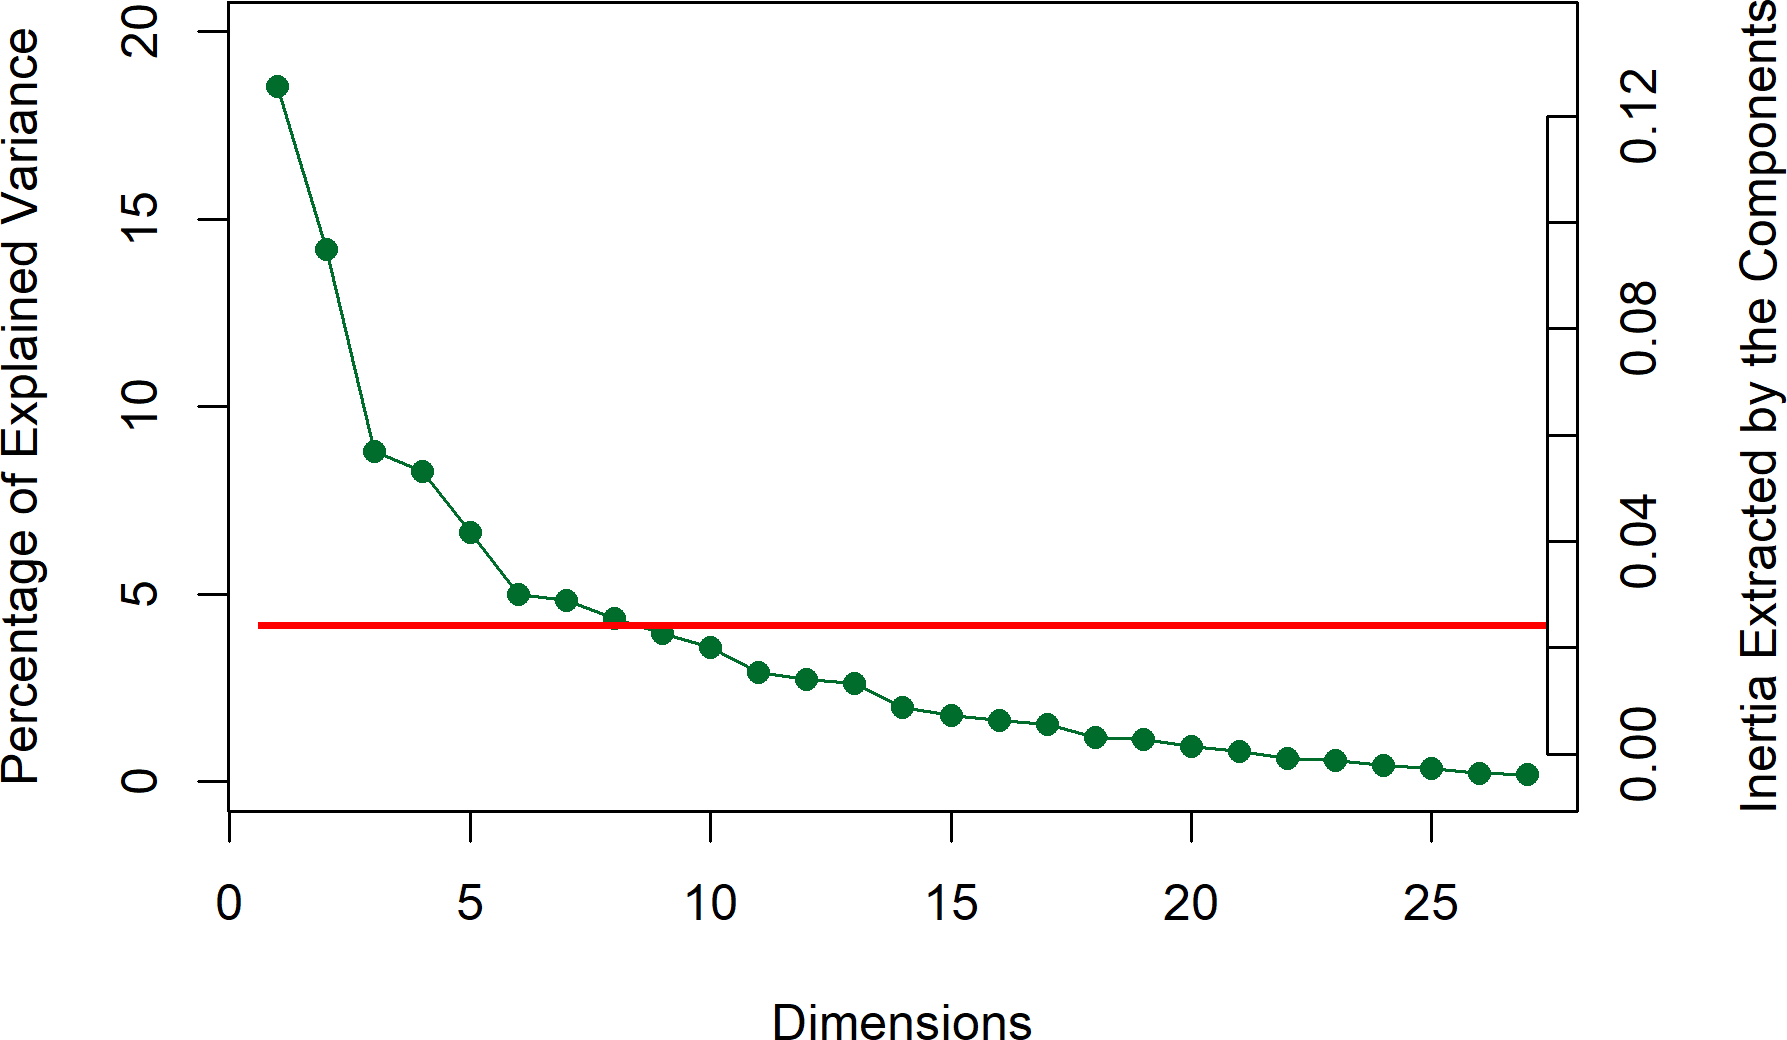
\includegraphics{./Music-Descriptor-Space_files/figure-latex/scree4excerptsq-1.png}
  \caption*{\footnotesize \textit{Note.} The horizontal line indicates the average variance extracted per dimension. }\label{fig:scree4excerptsq}  
 \end{center}
\end{wrapfigure}

\hypertarget{excerpts}{%
\subsubsection{Excerpts}\label{excerpts}}

The results of the CA performed on the contingency table revealed two significant dimensions, accounting for 32.74\% of the total variance. Figure \ref{fig:scree4excerptsq} displays the scree plot, which shows for this analysis the percentage of variance explained by each dimension.

Preliminary plots of the factor scores obtained from the CA revealed that Excerpts 6 and 14 distorted the factor space, with these two excerpts dominating the second and third dimensions. To help interpret the factor space, these two excerpts were removed from the data and the CA was recomputed. Excerpts 6 and 14 were then added back in as \emph{supplementary observations}, a technique which visualizes the information these elements share with the elements retained in the main sample without distorting the factor space. The proximity of these supplementary observations to the origin helps identify how much information is shared with the rest of the sample. The closer the supplementary observations are to the origin, the less information they share with the rest of the sample.

The HCA performed on the row factor scores of the CA revealed four clusters of excerpts (see supplementary materials for the tree diagram). Figure \ref{fig:factormapsQ} displays the first two factorial dimensions and the row factor scores calculated by the CA, colored according to the clusters revealed by the HCA, with Excerpts 6 and 14 as supplementary observations colored separately. Figure \ref{fig:factormapsQ} also displays the column factor scores for the qualities calculated by the CA (right), with the levels of a given quality colored the same. For clarity, only the levels of qualities that contributed significantly (see below, and Figure \ref{fig:contributionsQ}) are displayed.

The proximity between two points in Figure \ref{fig:factormapsQ} indicates their similarity when these points are on the same map. Because the CA computes a space common to both rows and columns, points on different maps can also be compared. Proximity between points on separate maps reflects their association relative to the average, for example Excerpt 24 is more associated with Legato articulation than is the average excerpt (Abdi \& Williams, 2010).

\begin{figure}   
  \centering  
  \caption{CA: Musical Qualities Survey, factor plots for Excerpts, colored according to clusters identified by the HCA, and important musical qualities, colored such that levels of each quality are the same color.}
    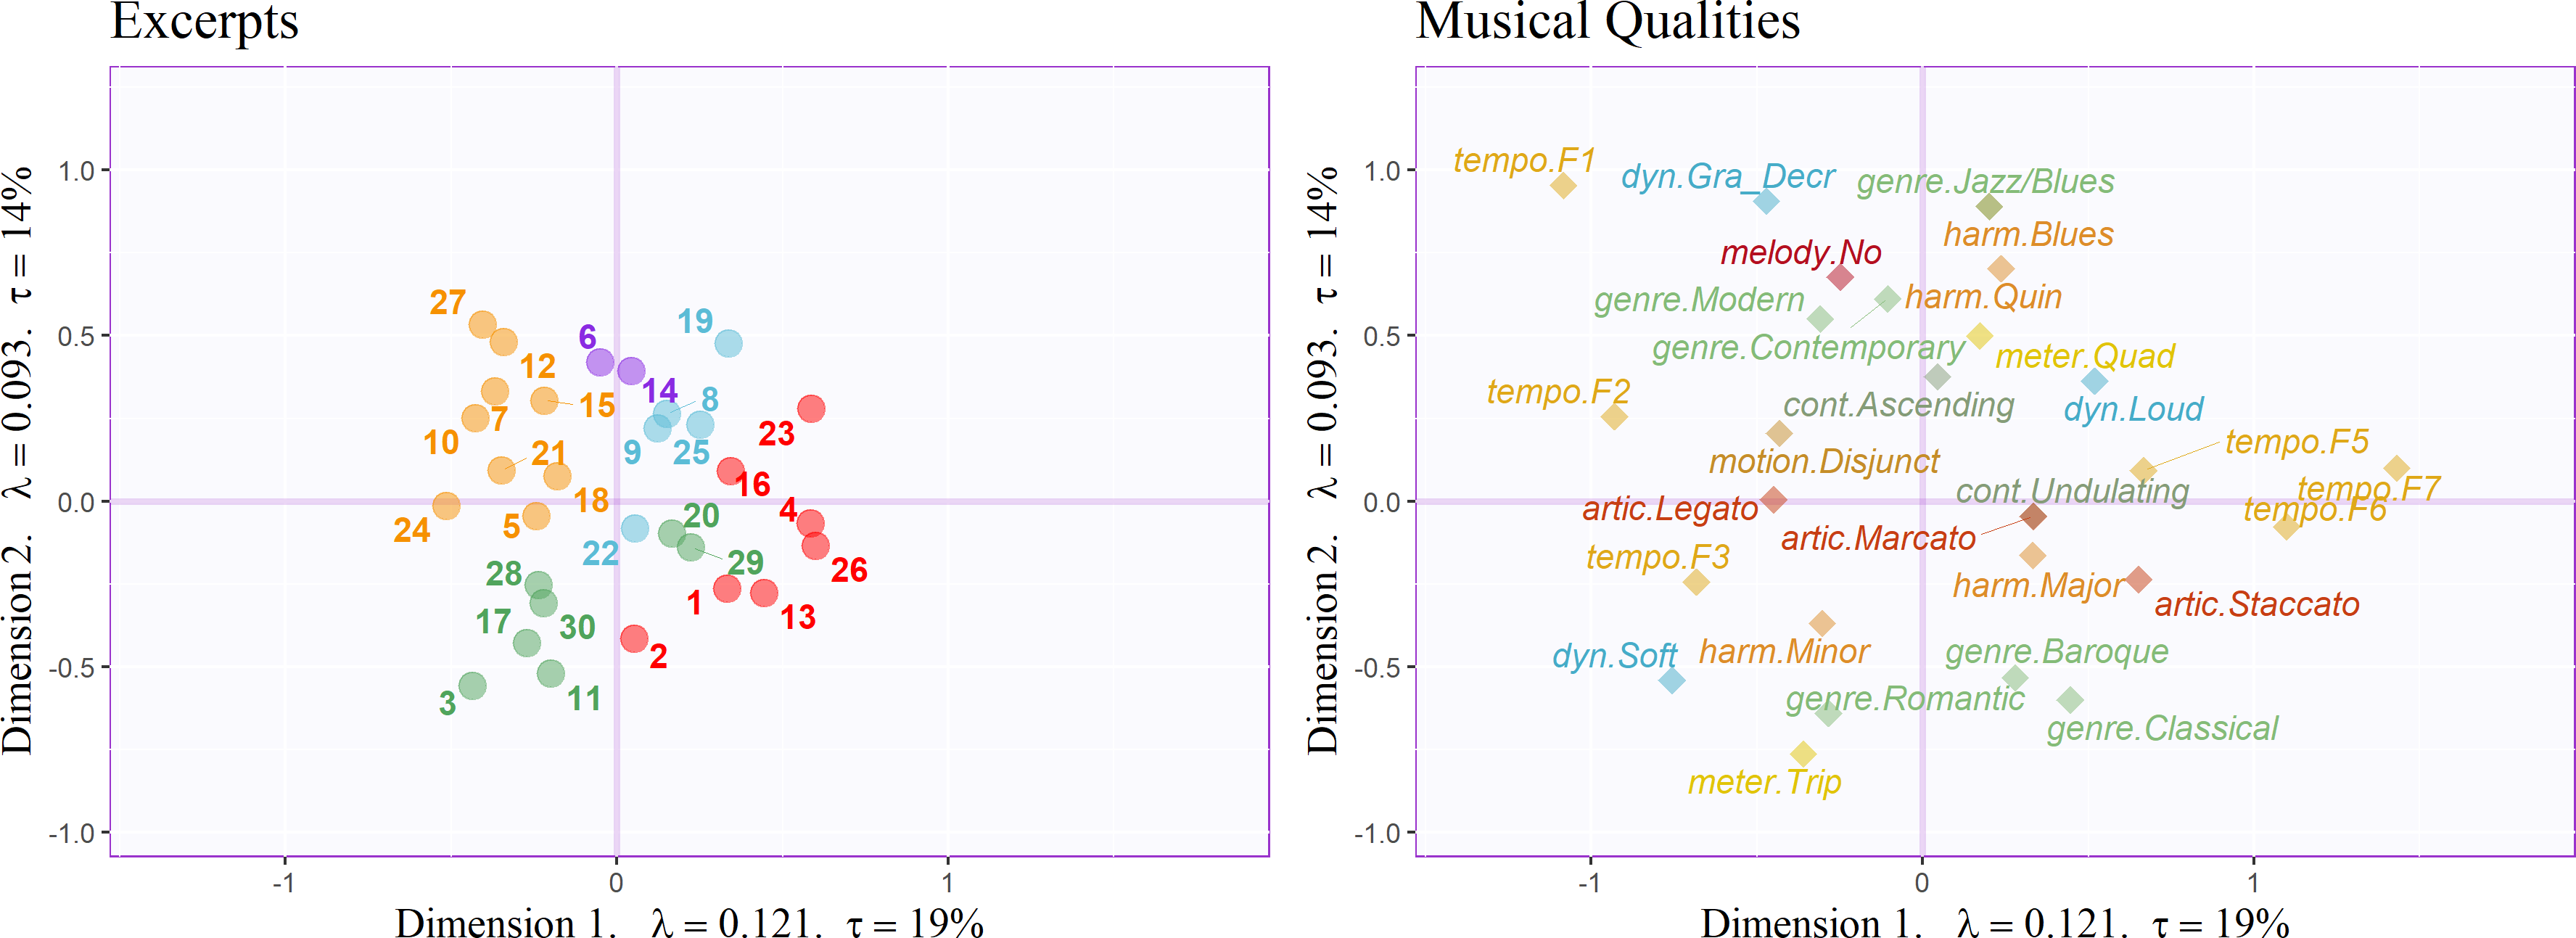
\includegraphics{./Music-Descriptor-Space_files/figure-latex/factormapsQcode-1.png}
  \label{fig:factormapsQ}
  \caption*{\footnotesize \textit{Note.} Axes are labeled with the dimension, eigenvalue, and the explained variance for the dimension. }
\end{figure}

To evaluate the relative importance of the excerpts and musical qualities in defining each dimension, we computed their \emph{contributions} to the dimensions. Contributions are similar to a squared coefficient of correlation and vary between zero and one with zero indicating no importance and one indicating maximum importance (Abdi \& Williams, 2010). Contributions---being squared---are positive, but to facilitate interpretation contributions are signed to express the sign of the factor scores. Contributions whose magnitude is larger than the average contribution are considered important for their factorial dimensions. A plot of the contributions for all excerpts and variables is in the supplementary materials.

Figure \ref{fig:contributionsQ} shows only the contributions of excerpts and qualities important for the first two dimensions. For Dimension 1---ordered by magnitude---Excerpts 26, 4, 23, and 13 contribute to the positive side of the dimension, whereas Excerpts 24, 3, 10, 27, and 7 contribute to the negative side of the dimension. Low tempi (tempo.F2 and tempo.F1) contribute to the negative side, along with legato (smooth) articulation and soft dynamics. Finally, high tempi contribute to the positive side, along with marcato (accented) and staccato (separate) articulations and loud dynamics. Single levels from other variables also contribute to the first dimension: major harmony, classical genre, and undulating contour in the positive direction and disjunct motion and triple meter in the negative direction.

For Dimension 2, Excerpts 27, 19, 12, 7, and 15 contribute to the positive side of the dimension, whereas Excerpts 3, 11, 17, and 2 contribute to the negative side. Newer genres (Contemporary, Jazz/Blues, and Modern) contribute to the positive side of Dimension 2, along with Blues and Quintal harmony, Quadruple meter, Gradual decrescendo and loud dynamics, ascending contour, ``no melody,'' and the slowest level of the tempo variable. Older genres (Baroque, Classical, and Romantic) contribute to the negative side of this dimension, along with soft dynamics, minor harmony, and triple meter.\footnote{A full list of contributions is available at the first author's GitHub, the URL for which is in the author note and the supplementary materials.}

\begin{figure}   
  \centering  
  \caption{CA: Musical Qualities survey, important signed contributions for the first two dimensions, colored similarly to Figure 3.}
    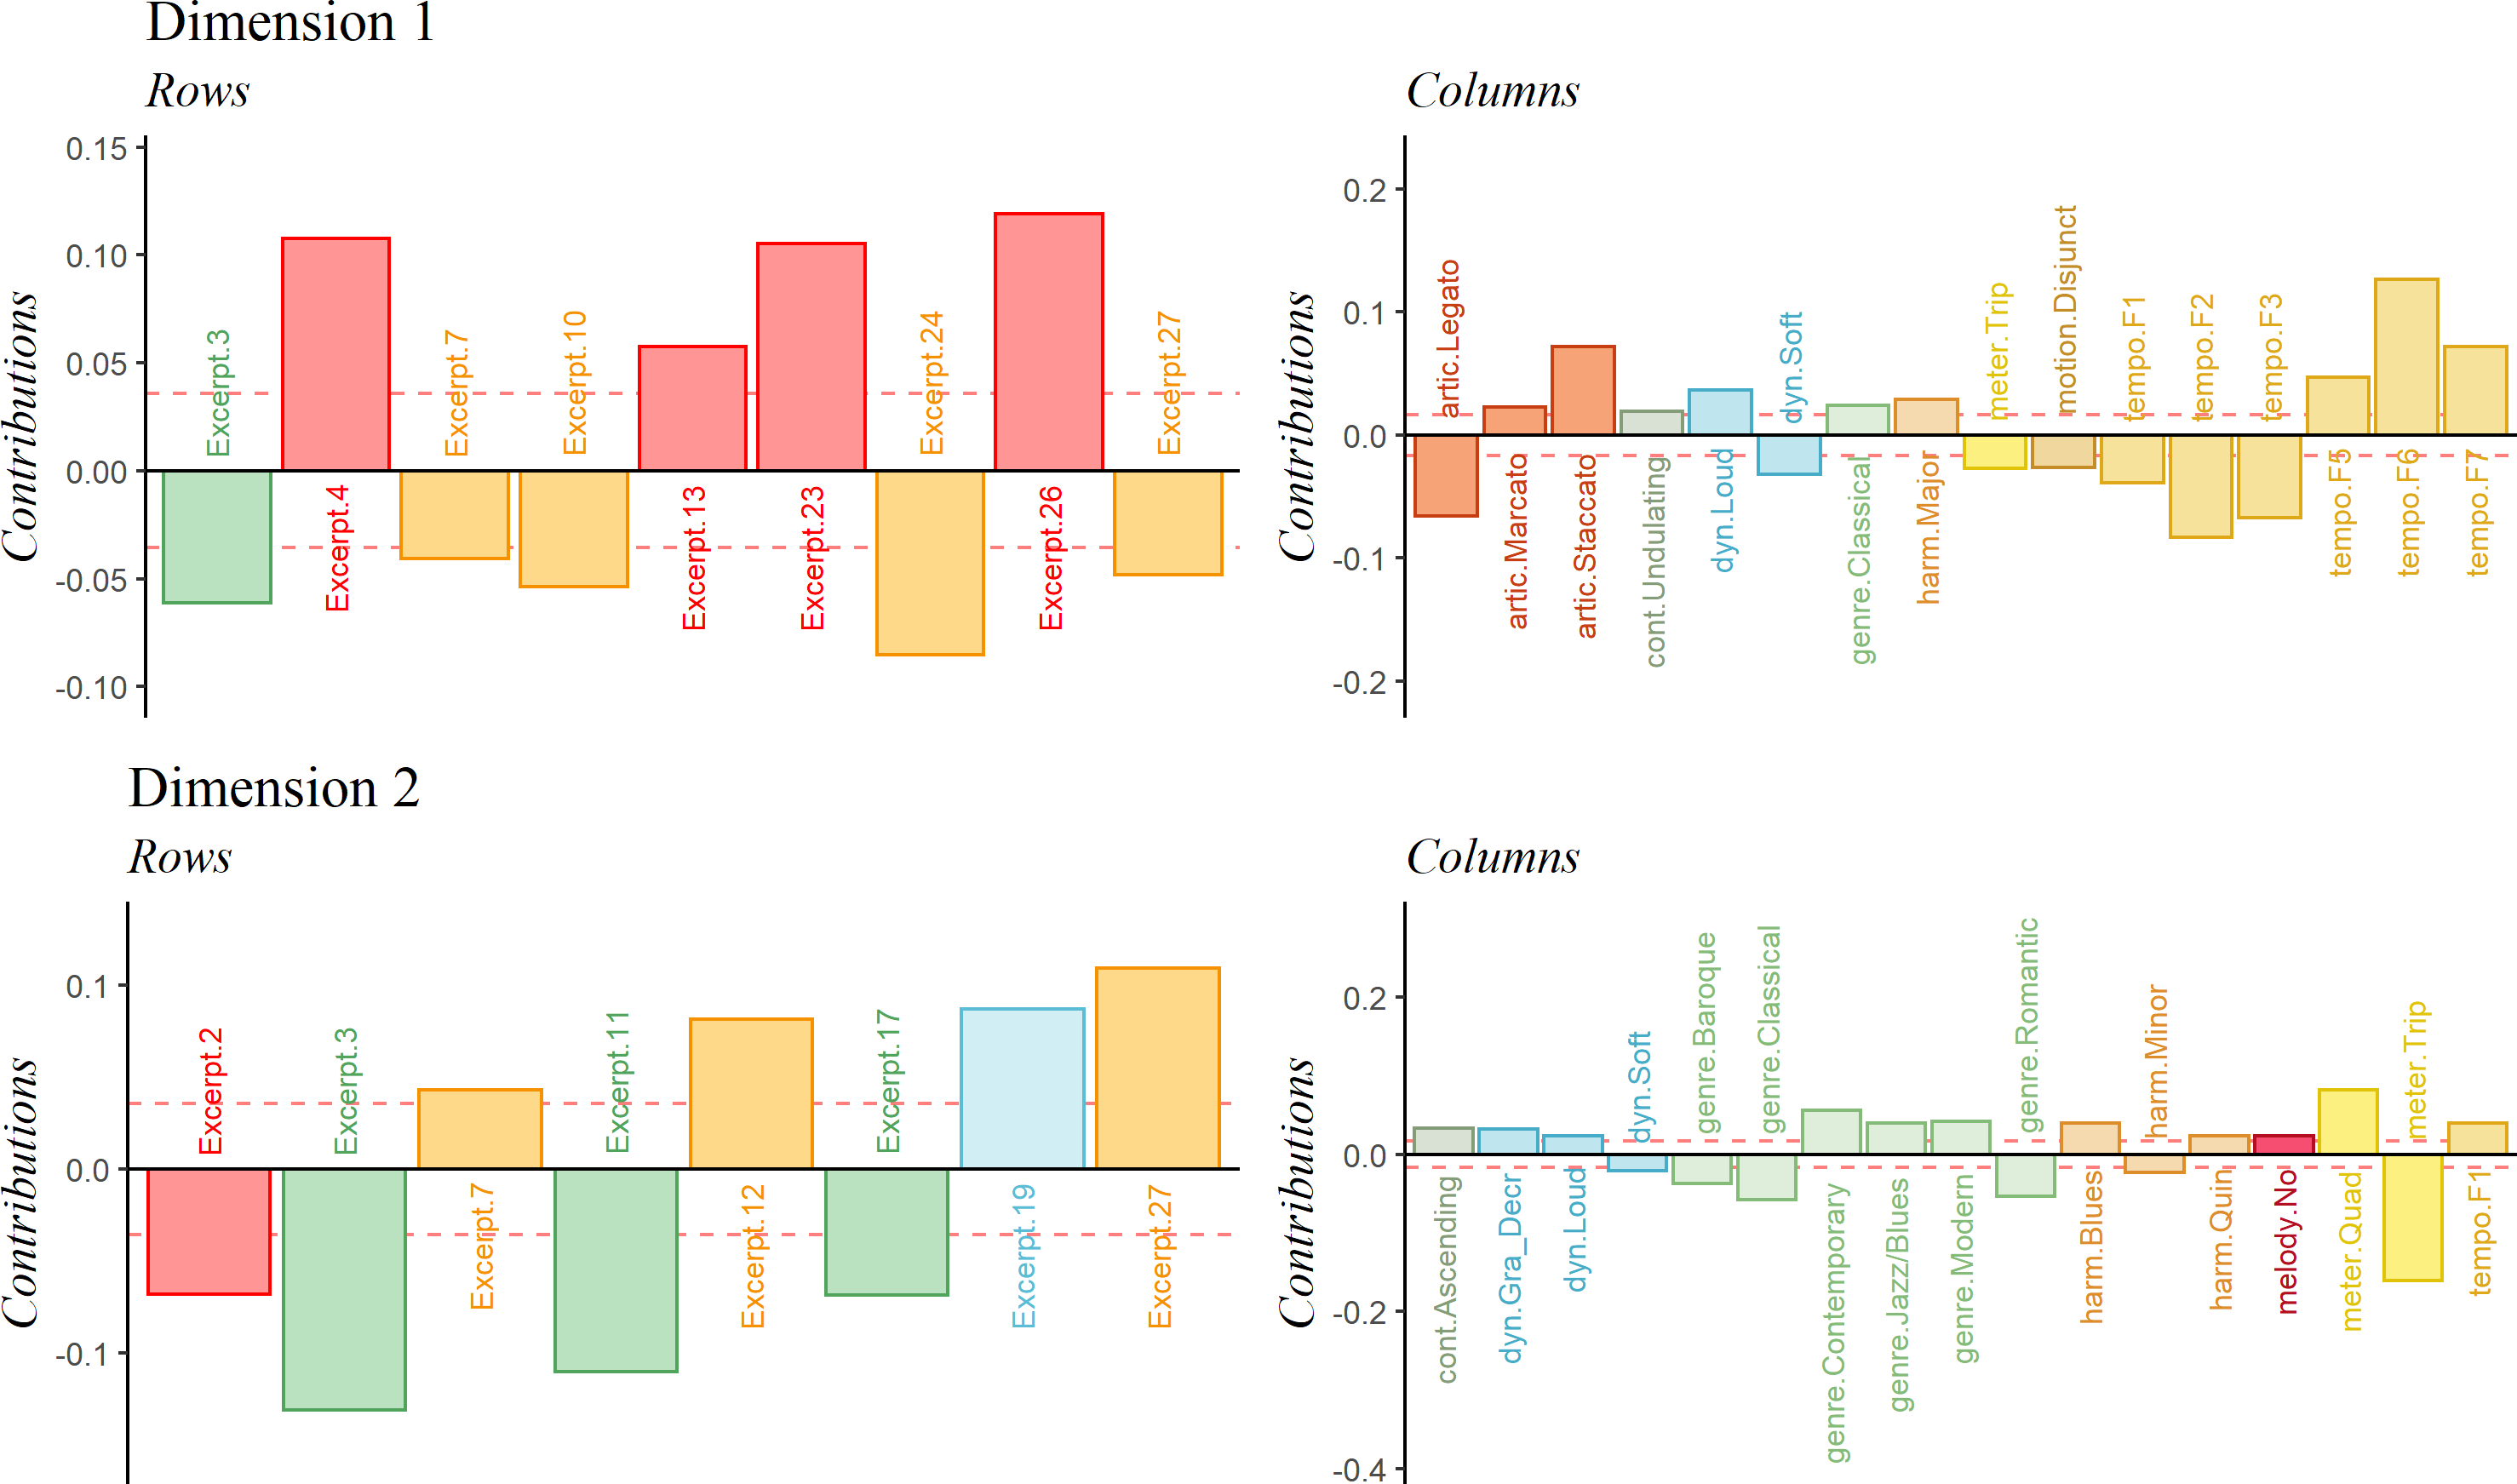
\includegraphics{./Music-Descriptor-Space_files/figure-latex/contributionsQcode-1.png}
  \label{fig:contributionsQ}
  \caption*{\footnotesize \textit{Note.} The y-axis represents the value of the contributions.}
\end{figure}

\hypertarget{experiment-1-discussion}{%
\subsection{Experiment 1 Discussion}\label{experiment-1-discussion}}

Observing no group differences between French and American participants in the results of the MDS on the co-occurrence matrix suggests that the trained musicians perceived the excerpts with which they were presented similarly.

The results of the CA (Figure \ref{fig:factormapsQ}) reveal a few musical connections: for example between tempo and articulation (on Dimension 1), and between genre and harmony (on Dimension 2). Staccato articulations, associated on this factor plot with high tempi, are played light and separate, and legato articulations, associated with slow tempi, are played smooth and connected. The coordinate mapping of jazz/blues harmony and genre, which are on top of one another, is the most extreme example of a genre being associated with certain harmonic material, but other connections are also revealed. The second dimension separates older styles, such as Baroque, Classical, and Romantic, from newer styles, Contemporary, Jazz/Blues, and Modern. Dimension 2 similarly separates harmonies associated with those styles, specifically older and simpler harmonies of major and minor from the more complex harmonies of Quintal and Blues.

The first dimension can be interpreted as arousal---tempo, articulation, and dynamics all load from greater arousal in the positive direction to lesser arousal in the negative direction on the first dimension. Dimension 2 is less clear, and does not seem to be tied to valence. Minor and major harmony, for example, both score negatively on Dimension 2. Instead, Figure \ref{fig:contributionsQ} shows that while two levels of the meter variable are the most important for this dimension, that genre is also important, based on the number of levels of genre that contribute significantly to Dimension 2. Considering the contributions of the genre and the harmony variables, it may be that the second dimension represents complexity.

\hypertarget{experiment-2-musical-adjectives-survey}{%
\section{Experiment 2: Musical Adjectives Survey}\label{experiment-2-musical-adjectives-survey}}

\hypertarget{methods-1}{%
\subsection{Methods}\label{methods-1}}

\hypertarget{participants-2}{%
\subsubsection{Participants}\label{participants-2}}

Participants with self-reported normal hearing were recruited for Experiment 2 without regard to level of music training. Participants in the United States were recruited by the UT Dallas Psych Research Sign-up (SONA) System, by word of mouth, and by social media. French participants were recruited by word of mouth, email, and social media. Only participants who signed up via the SONA System were compensated (i.e., with research participation credit). Out of 520 survey responses received, 166 were incomplete and removed. The remaining 354 were filtered by nationality: American participants who answered the question ``What's your nationality?'' with a compound nationality including American were retained, but those who indicated only a nationality other than American were excluded. ``Indian-American,'' for example, was included, but ``Ghanian,'' was not. This left a total of 278 (\(N\mathrm{_{France}}\) = 112, \(N\mathrm{_{USA}}\) = 166) survey responses for analysis. All recruitment measures were approved by the UT Dallas IRB.

\hypertarget{stimuli-1}{%
\subsubsection{Stimuli}\label{stimuli-1}}

The stimuli used for Experiment 2 are the same as those used for Experiment 1.

\hypertarget{survey-1}{%
\subsubsection{Survey}\label{survey-1}}

The procedure for participants in Experiments 1 and 2 was similar. Participants received a link to a Qualtrics survey presented in either English or French, depending on the country in which they were recruited, and instructions regarding listening environment were the same as in Experiment 1. After standard informed consent procedures, participants listened to 15 of the 30 excerpts, presented one at a time, in a random order, and performed a CATA task. Participants were instructed to select any and all adjectives that they felt described the stimulus. Participants were provided with a list of 33 adjectives, presented in a random order for each stimulus, such as such as ``Dark,'' ``Warm,'' and ``Colorful'' (French: ``Sombre,'' ``Chaleureux,'' and ``Coloré''). The adjectives for this survey were selected using Wallmark (2019) as a guide and in consultation with a French professional musician. Some adjectives were initially selected in French and some in English. In all cases, adjectives were selected for which there was a clear French (vis-à-vis English) translation. The adjectives are listed in English and in French in the supplementary materials. Following the experimental task, the participants were asked to provide demographic data, including age, gender identity, nationality, occupation, and musical experience.

\hypertarget{data-processing-analysis}{%
\subsubsection{Data Processing \& Analysis}\label{data-processing-analysis}}

Data for the survey for Experiment 2 were processed similarly to Experiment 1. Due to a technical error, French participants were not presented with Excerpt 17, so the data for that excerpt were removed from the dataset for the American participants. Although excerpts 6 and 14 were removed from Experiment 1 data for being outliers, they were not found to be outliers in Experiment 2, and were therefore included in all of the analyses for for this experiment. To process the data, first, all French survey responses were translated into English. Both sets of responses were then converted into ``bricks'' of data, with the excerpts on the rows, the adjectives on the columns, and participants on the pages. On a page, at the intersection of a row and column was a one or a zero, with a one indicating that this participant had selected this adjective (column) to describe this stimulus (row). The bricks were then summed across pages to obtain a pseudo-contingency table in which the intersection of a row and a column stored the number of participants who selected an adjective to describe an excerpt.

To analyze the similarity structure between participants, we computed a co-occurrence matrix from the brick with participants on the rows and columns, such that the intersection of a row and column represented the number of common choices between participants. This co-occurrence matrix was then analyzed using MDS.

To analyze the excerpts and adjectives and obtain the music quality space, we performed a CA on the excerpts by adjectives contingency table. To identify potential clusters of excerpts or adjectives, two separate HCAs were computed, one on the row factor scores (excerpts) and one on the column factor scores (adjectives) obtained from the CA.

\begin{figure}   
  \centering  
  \caption{MFA: Data manipulation flowchart.}
    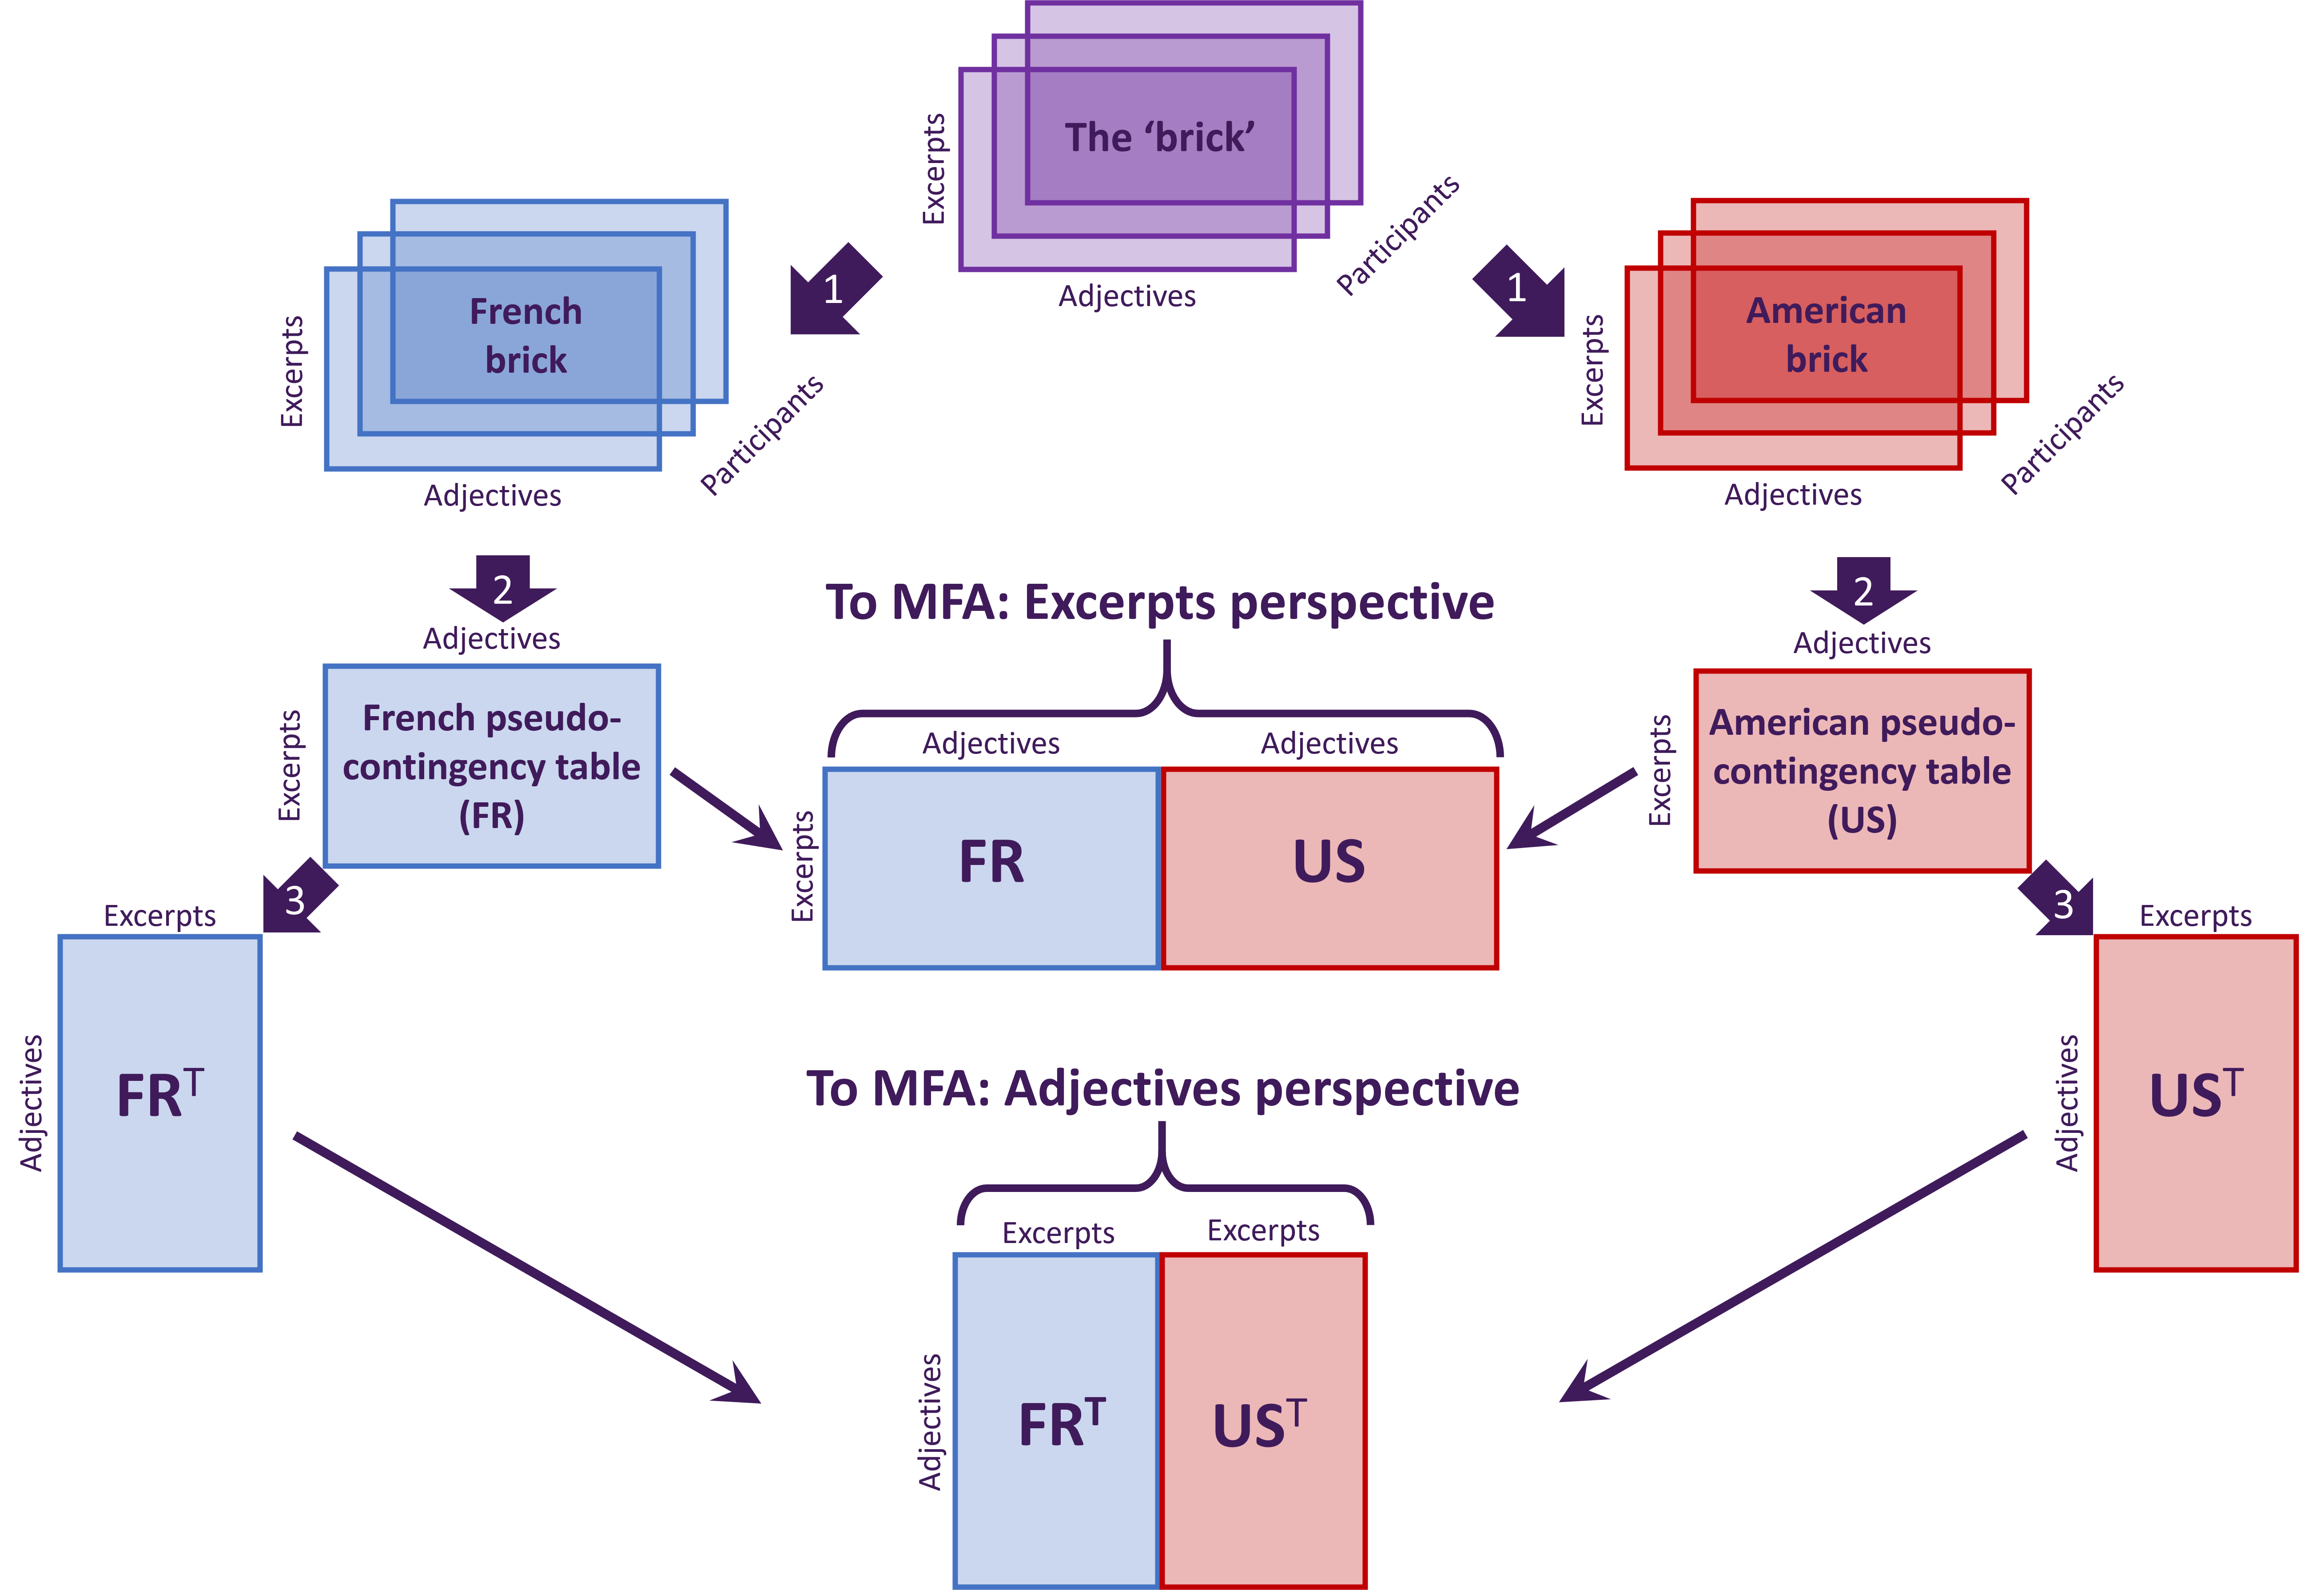
\includegraphics[width=1\columnwidth]{./Music-Descriptor-Space_files/figure-latex/mfadataflow.png}
  \label{fig:mfadataflow}
  \caption*{\footnotesize \textit{Note.} 1. Brick separated by nationality. 2. Separate bricks summed across pages. 3. Tables transposed. Thin arrows: tables as blocks concatenated into large matrices and sent to MFA for analysis.}
\end{figure}

We performed two MFAs, one to explore differences between French and American participants from the perspective of their use of adjectives, and another to explore differences between French and American participants from the perspective of their descriptions of excerpts. To prepare the data for these MFAs, we separated the brick into two separate bricks, one for the French participants and one for the American participants. These were each summed to obtain excerpts by adjectives pseudo-contingency tables for each nationality. These tables were then transposed to obtain adjectives by excerpts pseudo contingency tables for each group. The French and American excerpts by adjectives tables were then concatenated into a single large matrix in which each table represented a block, as were the transposed (adjectives by excerpts) tables. We then performed separate MFAs on each of these large matrices. Figure \ref{fig:mfadataflow} sketches the data manipulation process.

\hypertarget{results-1}{%
\subsection{Results}\label{results-1}}

\hypertarget{excerpts-1}{%
\subsubsection{Excerpts}\label{excerpts-1}}

\begin{wrapfigure}{h}{.4\textwidth}  
  \begin{center}
  \caption{CA: Scree plot for Adjectives Survey, showing percentage of explained variance per dimension.}
    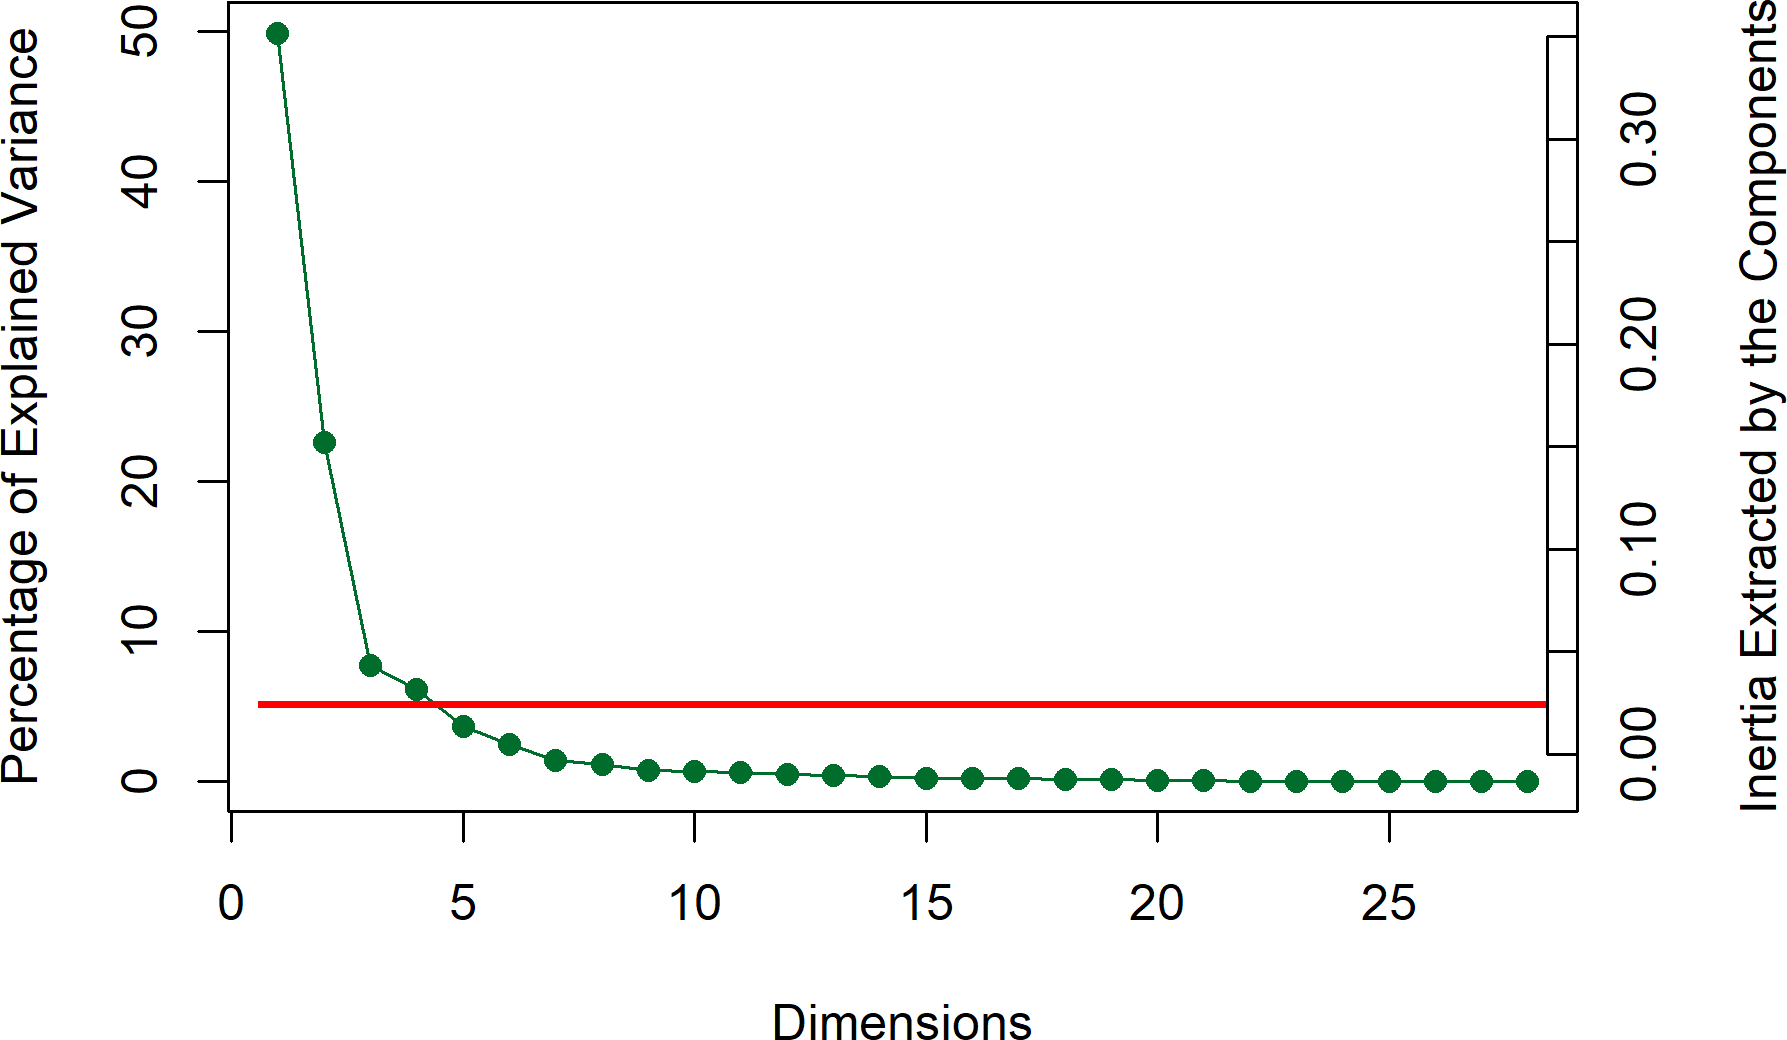
\includegraphics{./Music-Descriptor-Space_files/figure-latex/scree4descriptorscode-1.png}
  \caption*{\footnotesize \textit{Note.} Horizontal line indicates the average variance extracted per dimension. }\label{fig:scree4descriptors}  
 \end{center}
\end{wrapfigure}

\hypertarget{ca-hca}{%
\paragraph{CA \& HCA}\label{ca-hca}}

The CA performed on the AS pseudo-contingency table revealed two important dimensions, which together accounted for 72.55\% of the total variance (see Figure \ref{fig:scree4excerptsq}).

Figure \ref{fig:factormapsA} displays the factor scores for the excerpts and the adjectives. Interpretation of these plots is similar to the factor plots in Experiment 1. Because this experiment captures participant behavior relative to the descriptions of the excerpts, adjectives that are near one another can be interpreted as having been used similarly, such as ``Incisive'' and ``Complex.'' This plot shows a clear valence-arousal plane, such that the first dimension represents valence, with adjectives such as ``Sad'' and ``Dark'' on the right contrasting with ``Dancing'' and ``Happy'' on the left, and the second dimension represents arousal, such that ``Aggressive'' is contrasted near the top with ``Soft'' near the bottom. Similarly, Excerpts 27 and 26 are defined almost entirely by valence, with their projections on Dimension 1 accounting for 84\% and 86\% of their variance, respectively, and Excerpt 28 could be interpreted as being defined almost entirely by arousal, with its projection on Dimension 2 accounting for 81\% of its variance.

The HCAs computed separately on the factor scores for the rows (excerpts) and columns (adjectives) (see supplementary materials for tree diagrams) revealed four clusters for each set, and the excerpts and adjectives are colored according to these clusters for all plots for Experiment 2. The clusters of adjectives and excerpts identified by the HCA are grouped approximately by quadrant in Figure \ref{fig:factormapsA}, with the top right representing negative valence/high arousal, the top left representing positive valence/high arousal, the bottom left representing positive valence/low arousal, and the bottom right representing negative valence/low arousal. A few adjectives do not conform to this pattern---such as ``Monotonous'' and ``Dull''---because the factor scores for all dimensions were used for the HCA, and these adjectives were likely loading on higher dimensions.

\begin{figure}   
  \centering  
  \caption{CA: Adjectives survey, factor plots for Excerpts and Adjectives, each colored according to clusters identified by their respective HCAs}
    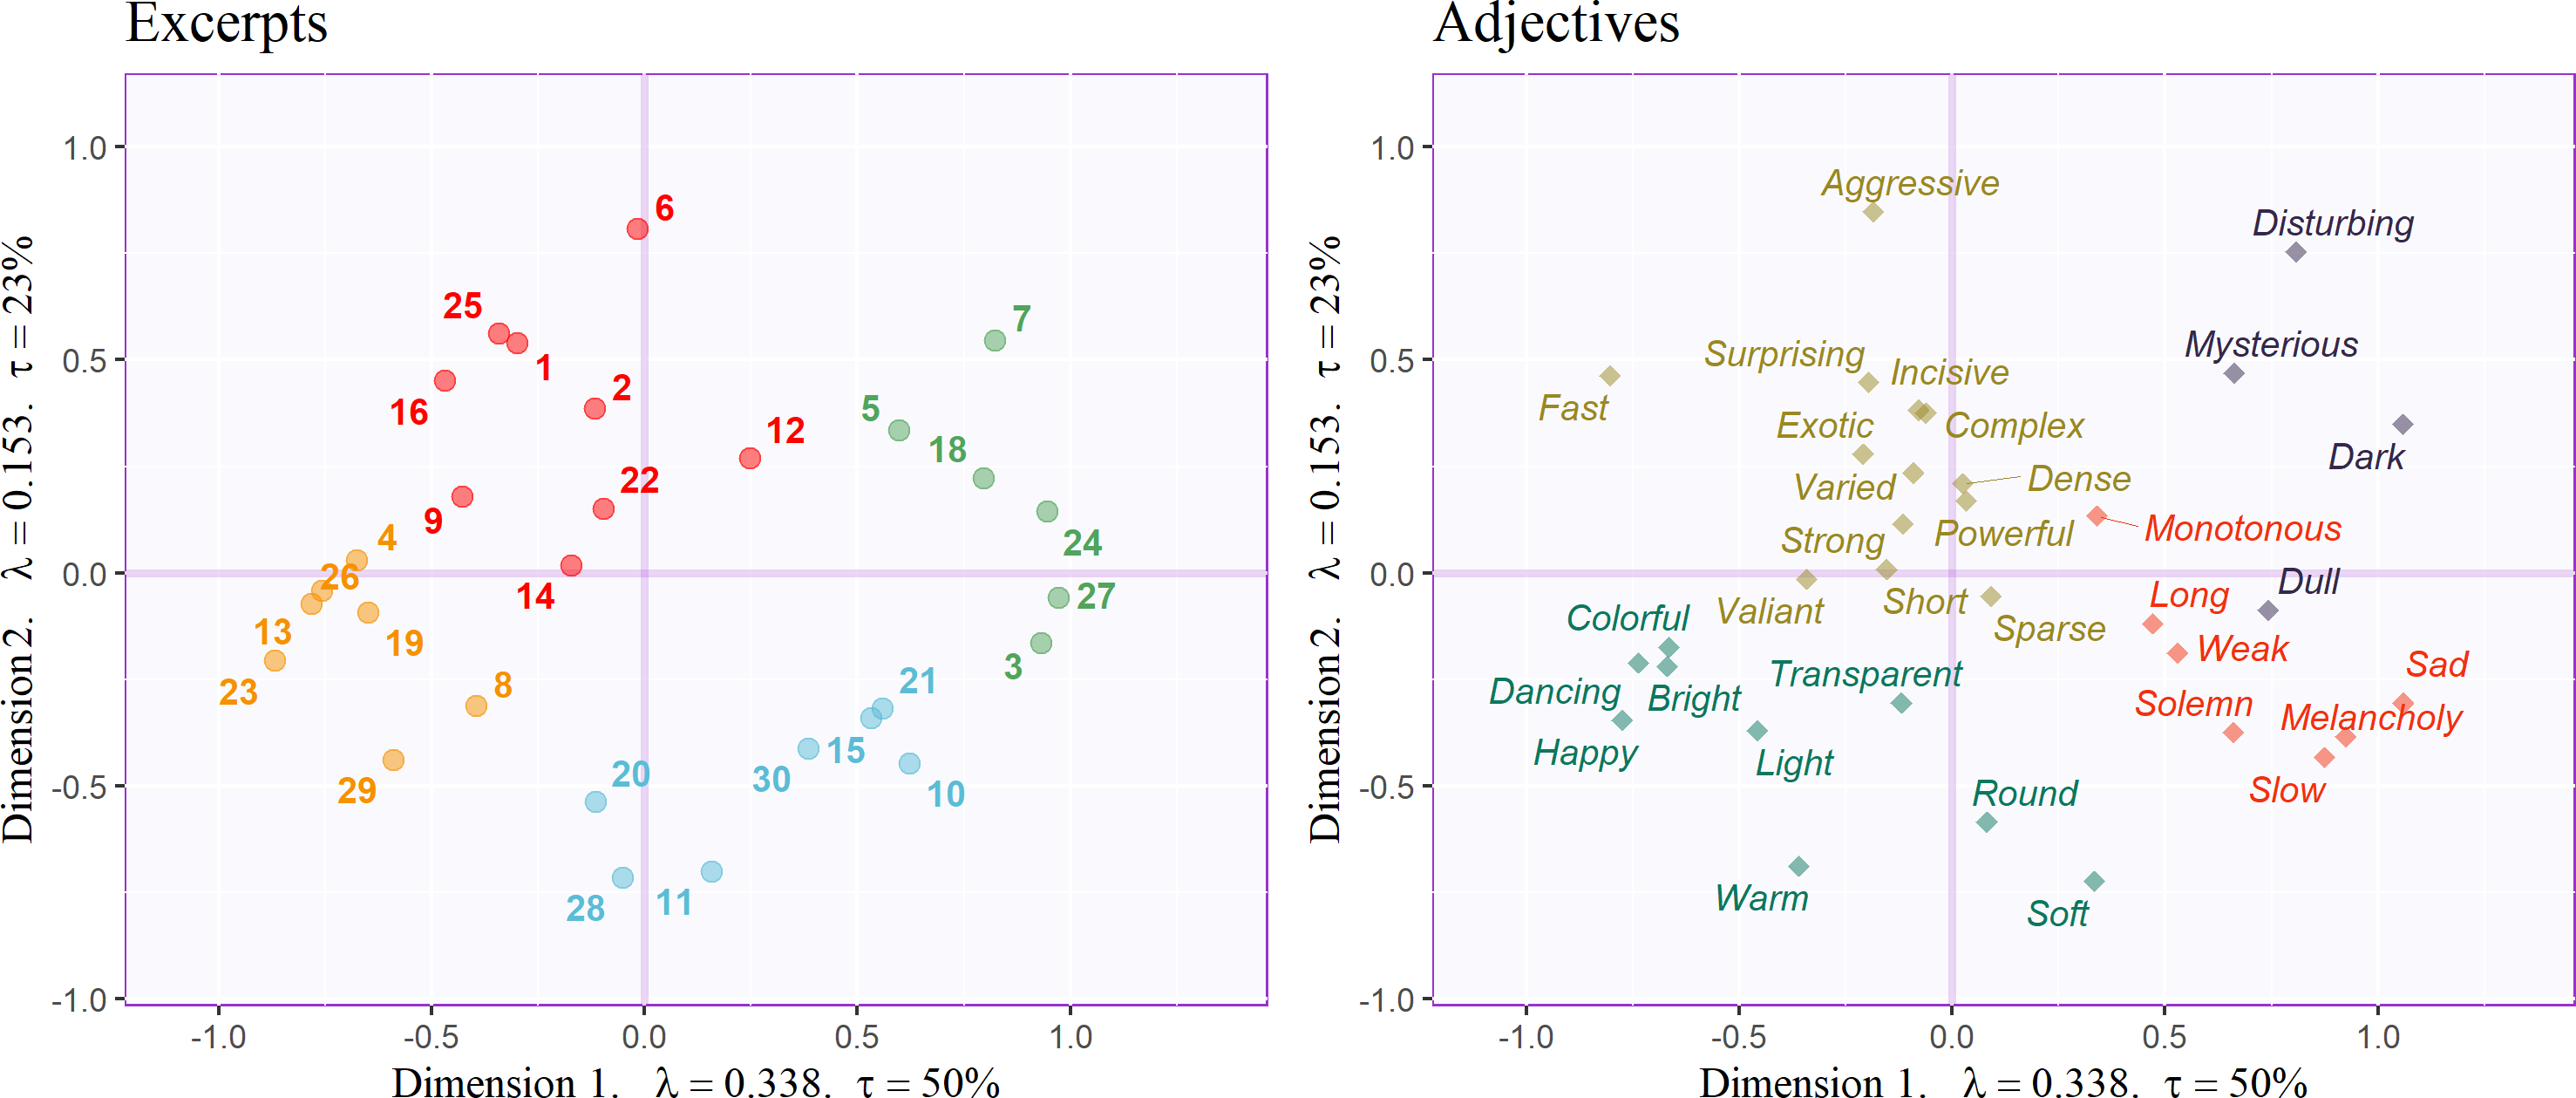
\includegraphics{./Music-Descriptor-Space_files/figure-latex/factormapsAcode-1.png}
  \label{fig:factormapsA}
  \caption*{\footnotesize \textit{Note.}  Axis labels indicate dimension, eigenvalue, and explained variance for that dimension.}
\end{figure}

Figure \ref{fig:contributionsA} displays the contributions of excerpts and adjectives important for the first two dimensions. For Dimension 1---in order of magnitude---Excerpts 27, 24, 3, 7, 18, and 10 contribute to the positive side of the dimension, whereas Excerpts 23, 13, 26, 4, and 19 contribute to the negative side. Adjectives ``Sad,'' ``Dark,'' ``Melancholy,'' ``Slow,'' ``Mysterious,'' ``Solemn,'' and ``Disturbing'' contribute in the positive direction, whereas ``Fast,'' ``Dancing,'' ``Happy,'' ``Colorful,'' and ``Bright'' contribute in the negative direction.

For Dimension 2, Excerpts 6, 1, 25, 7, and 16 contribute to the positive side of the dimension, whereas Excerpts 28, 11, 20, 29, and 10 contribute to the negative side. Adjectives ``Aggressive,'' ``Fast,'' ``Mysterious,'' ``Disturbing,'' and ``Complex'' contribute to the positive side of Dimension 2, whereas ``Warm,'' ``Soft,'' ``Slow,'' ``Round,'' Happy," ``Melancholy,'' and ``Solemn'' contribute to the negative side.

\begin{figure}   
  \centering  
  \caption{CA: Adjectives survey. Important signed contributions from rows and columns, colored according to clusters identified by their respective HCAs.}
    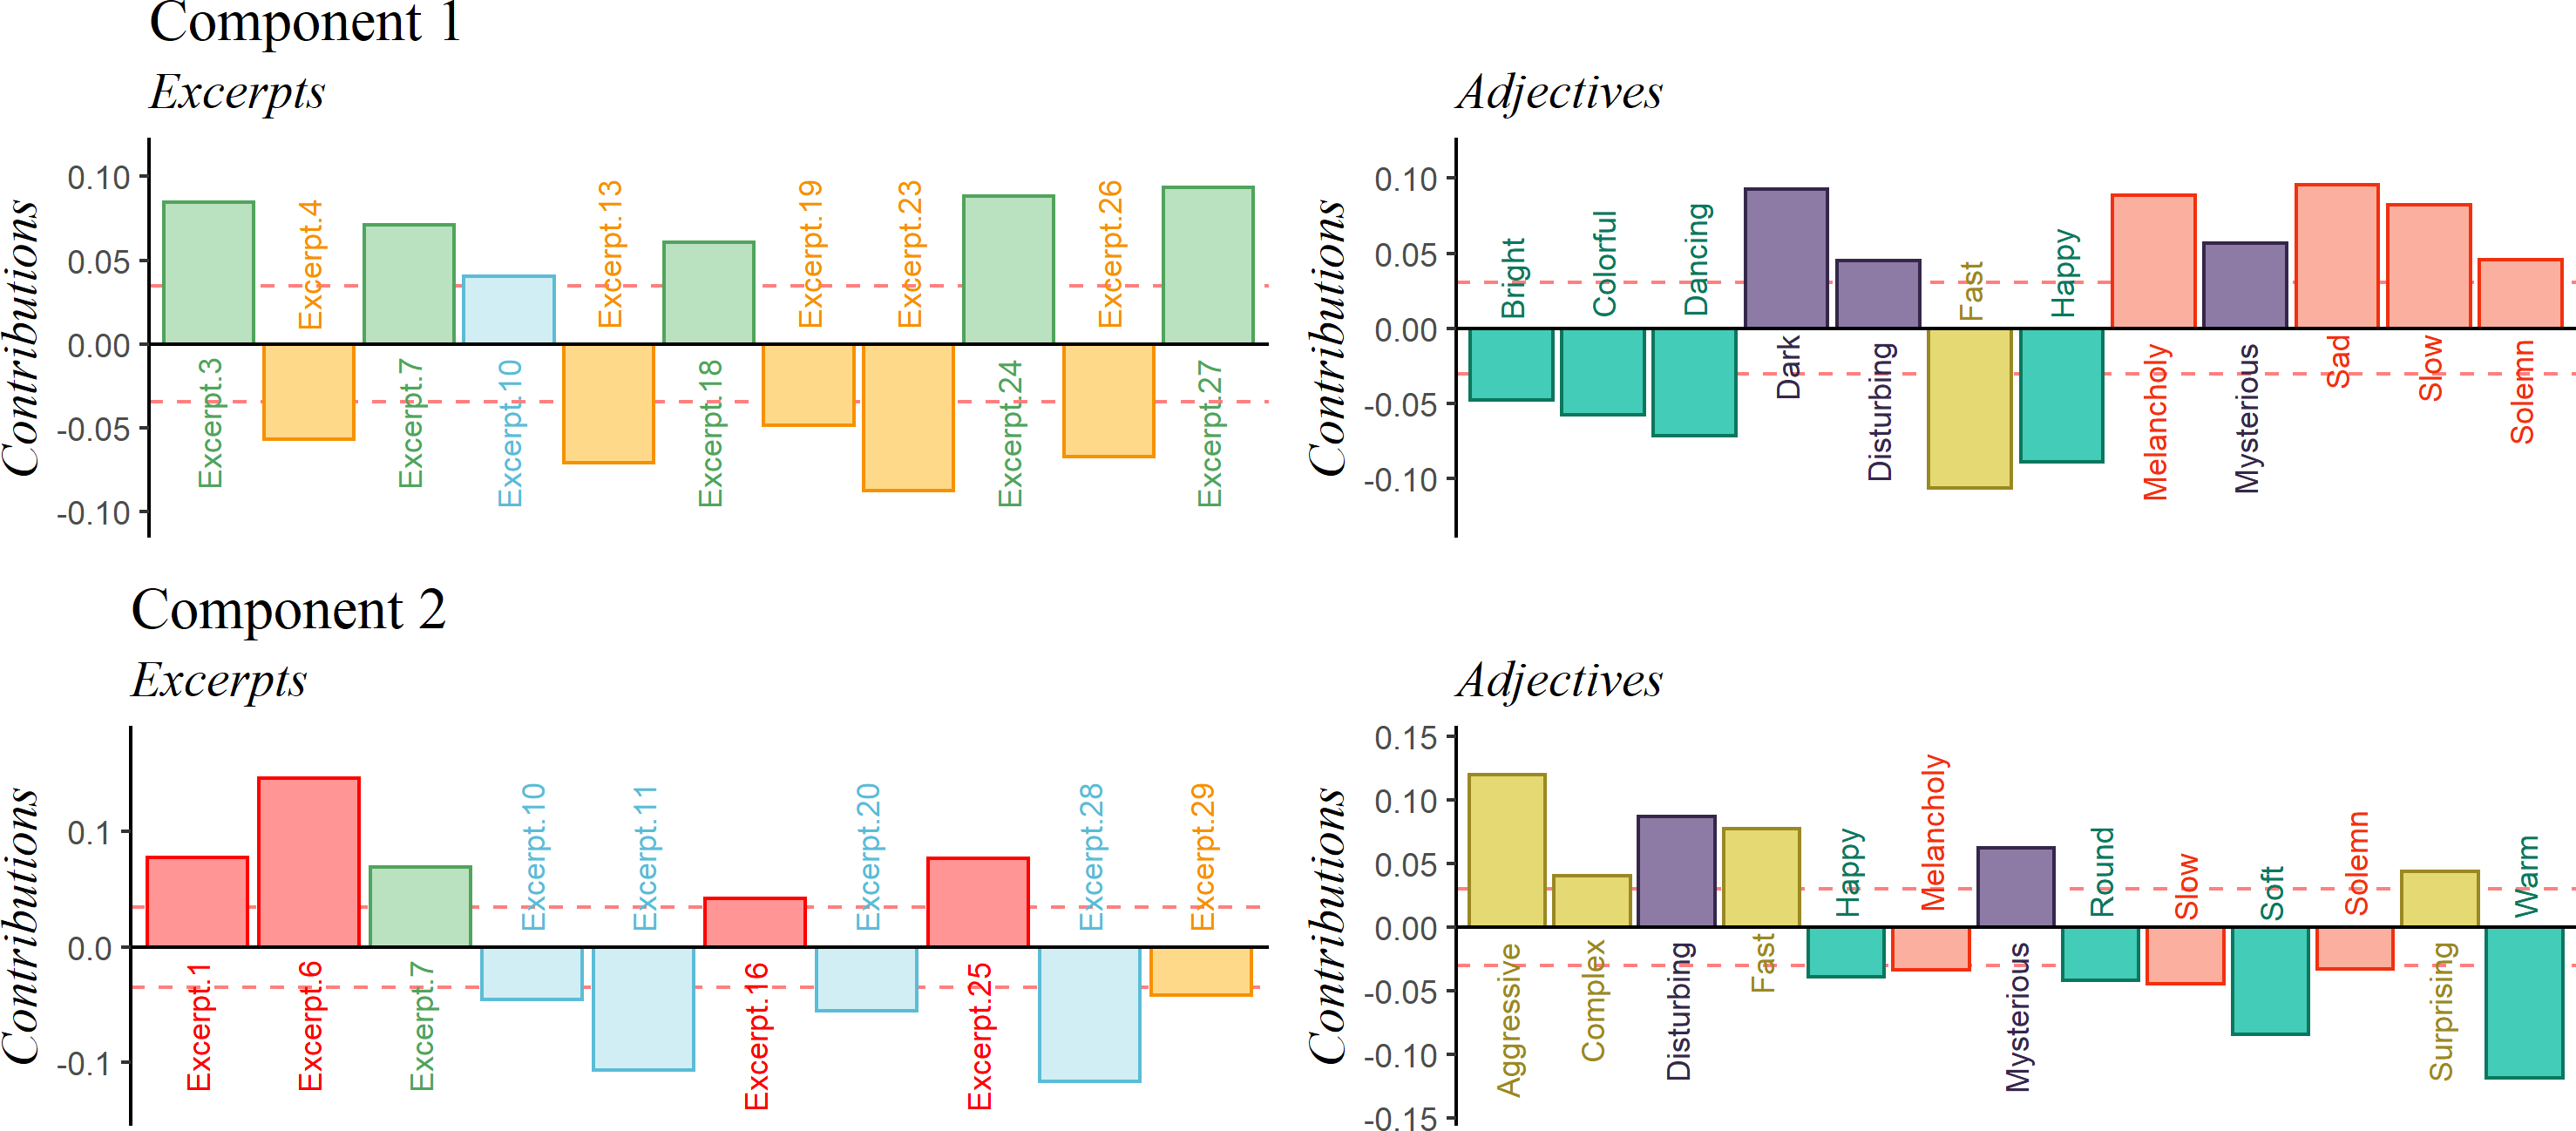
\includegraphics{./Music-Descriptor-Space_files/figure-latex/contributionsAcode-1.png}
  \label{fig:contributionsA}
  \caption*{}
\end{figure}

\hypertarget{participants-3}{%
\subsubsection{Participants}\label{participants-3}}

%\begin{wrapfigure}{h}{.4\textwidth}  
%  \begin{center}
%    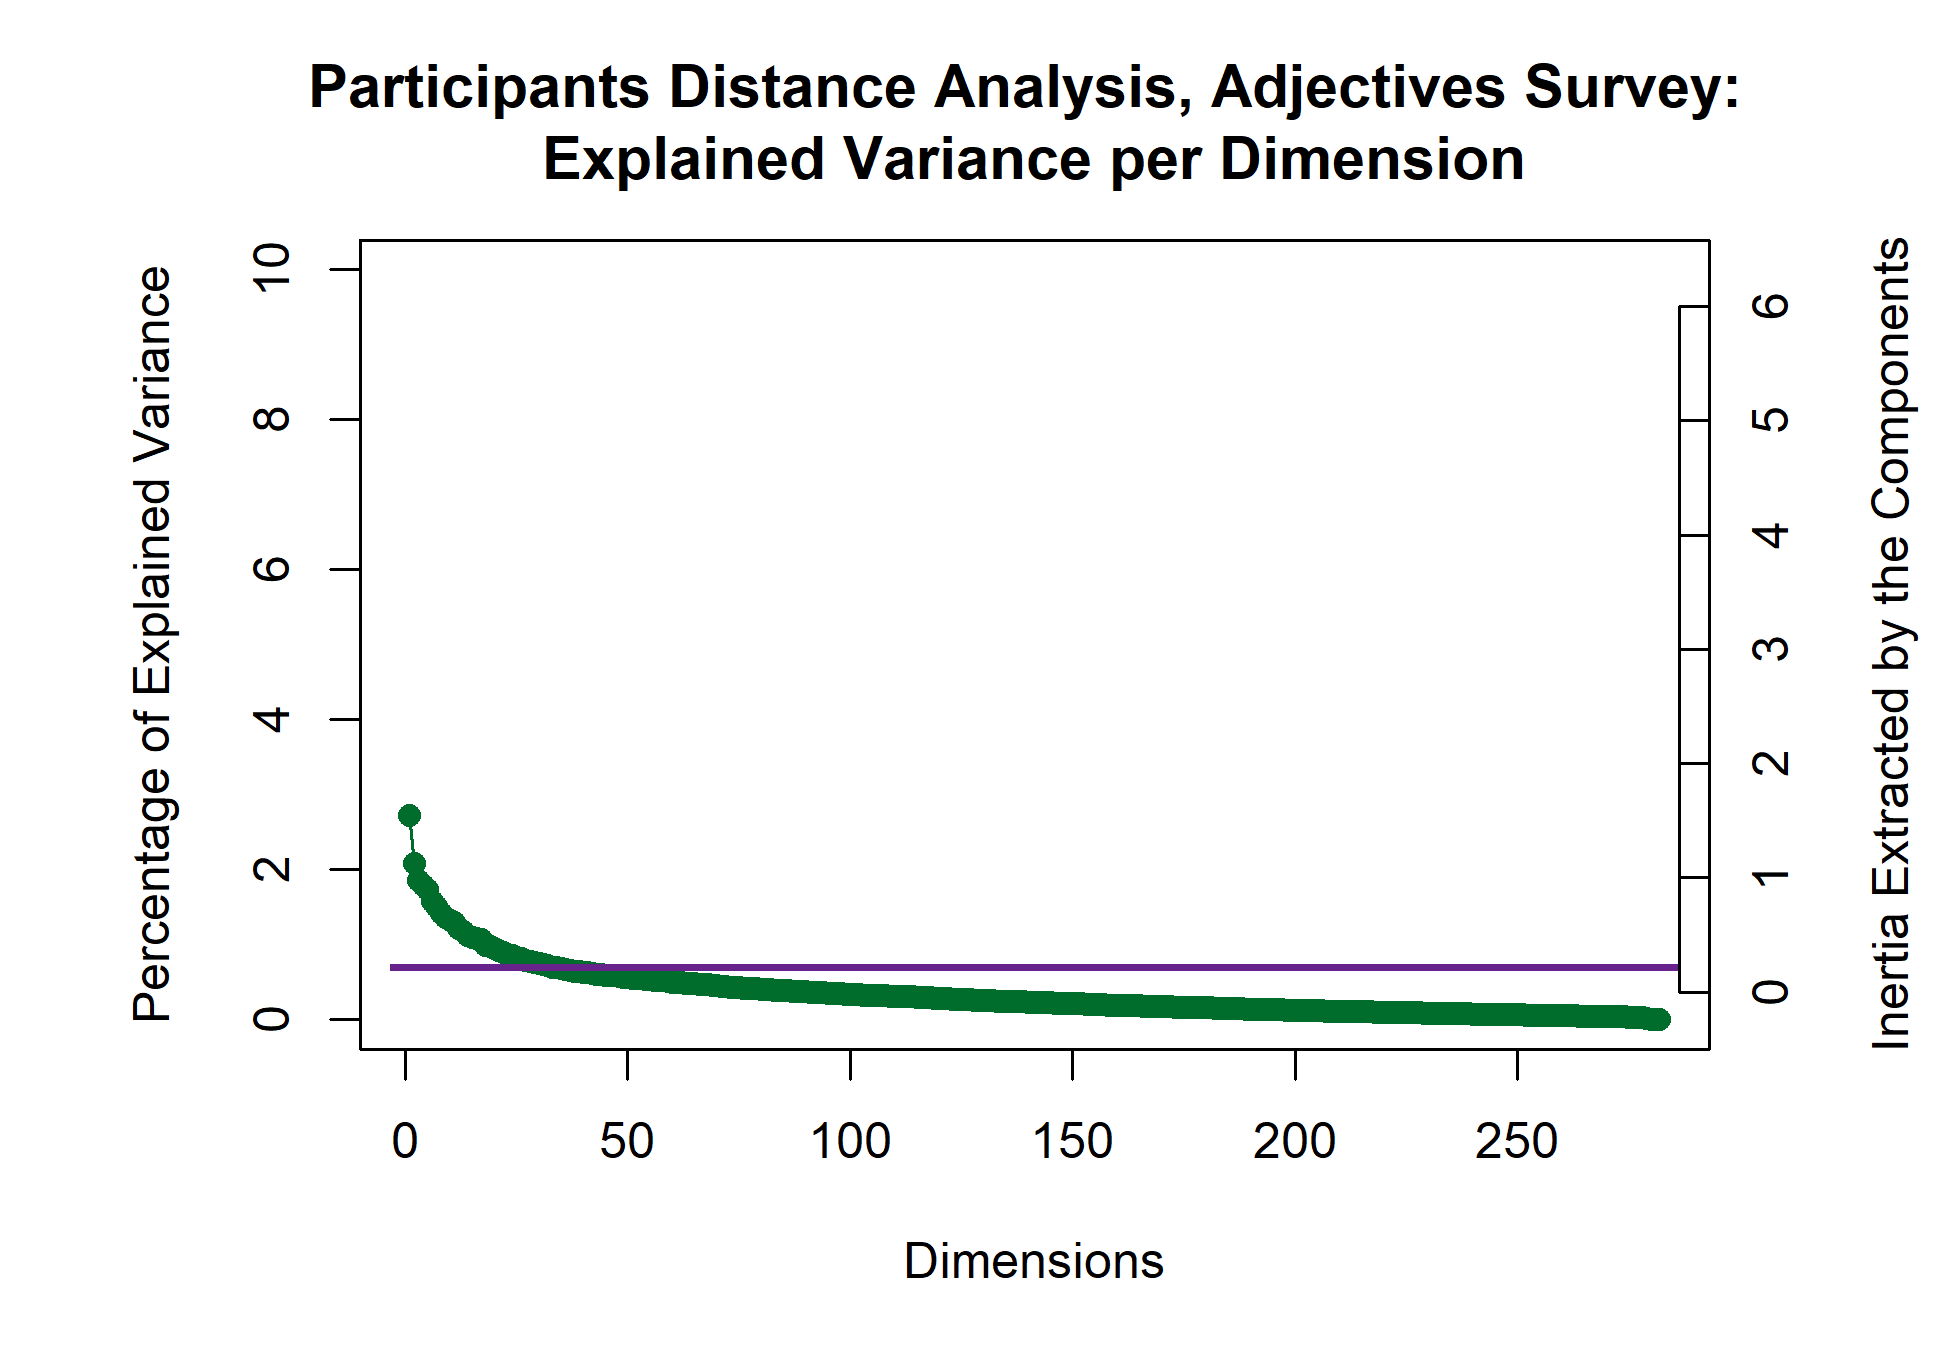
\includegraphics{./Music-Descriptor-Space_files/figure-latex/a.part.scree-1.png}
%  \caption{This plot shows the explained variance per dimension for this analyisis.}\label{fig:apartscree}  
% \end{center}
%\end{wrapfigure}

\begin{figure}   
  \centering  
  \caption{MDS: Distance analysis of the co-occurence matrix for the adjectives survey, including group means and bootstrap-derived confidence intervals, colored by nationality.}
    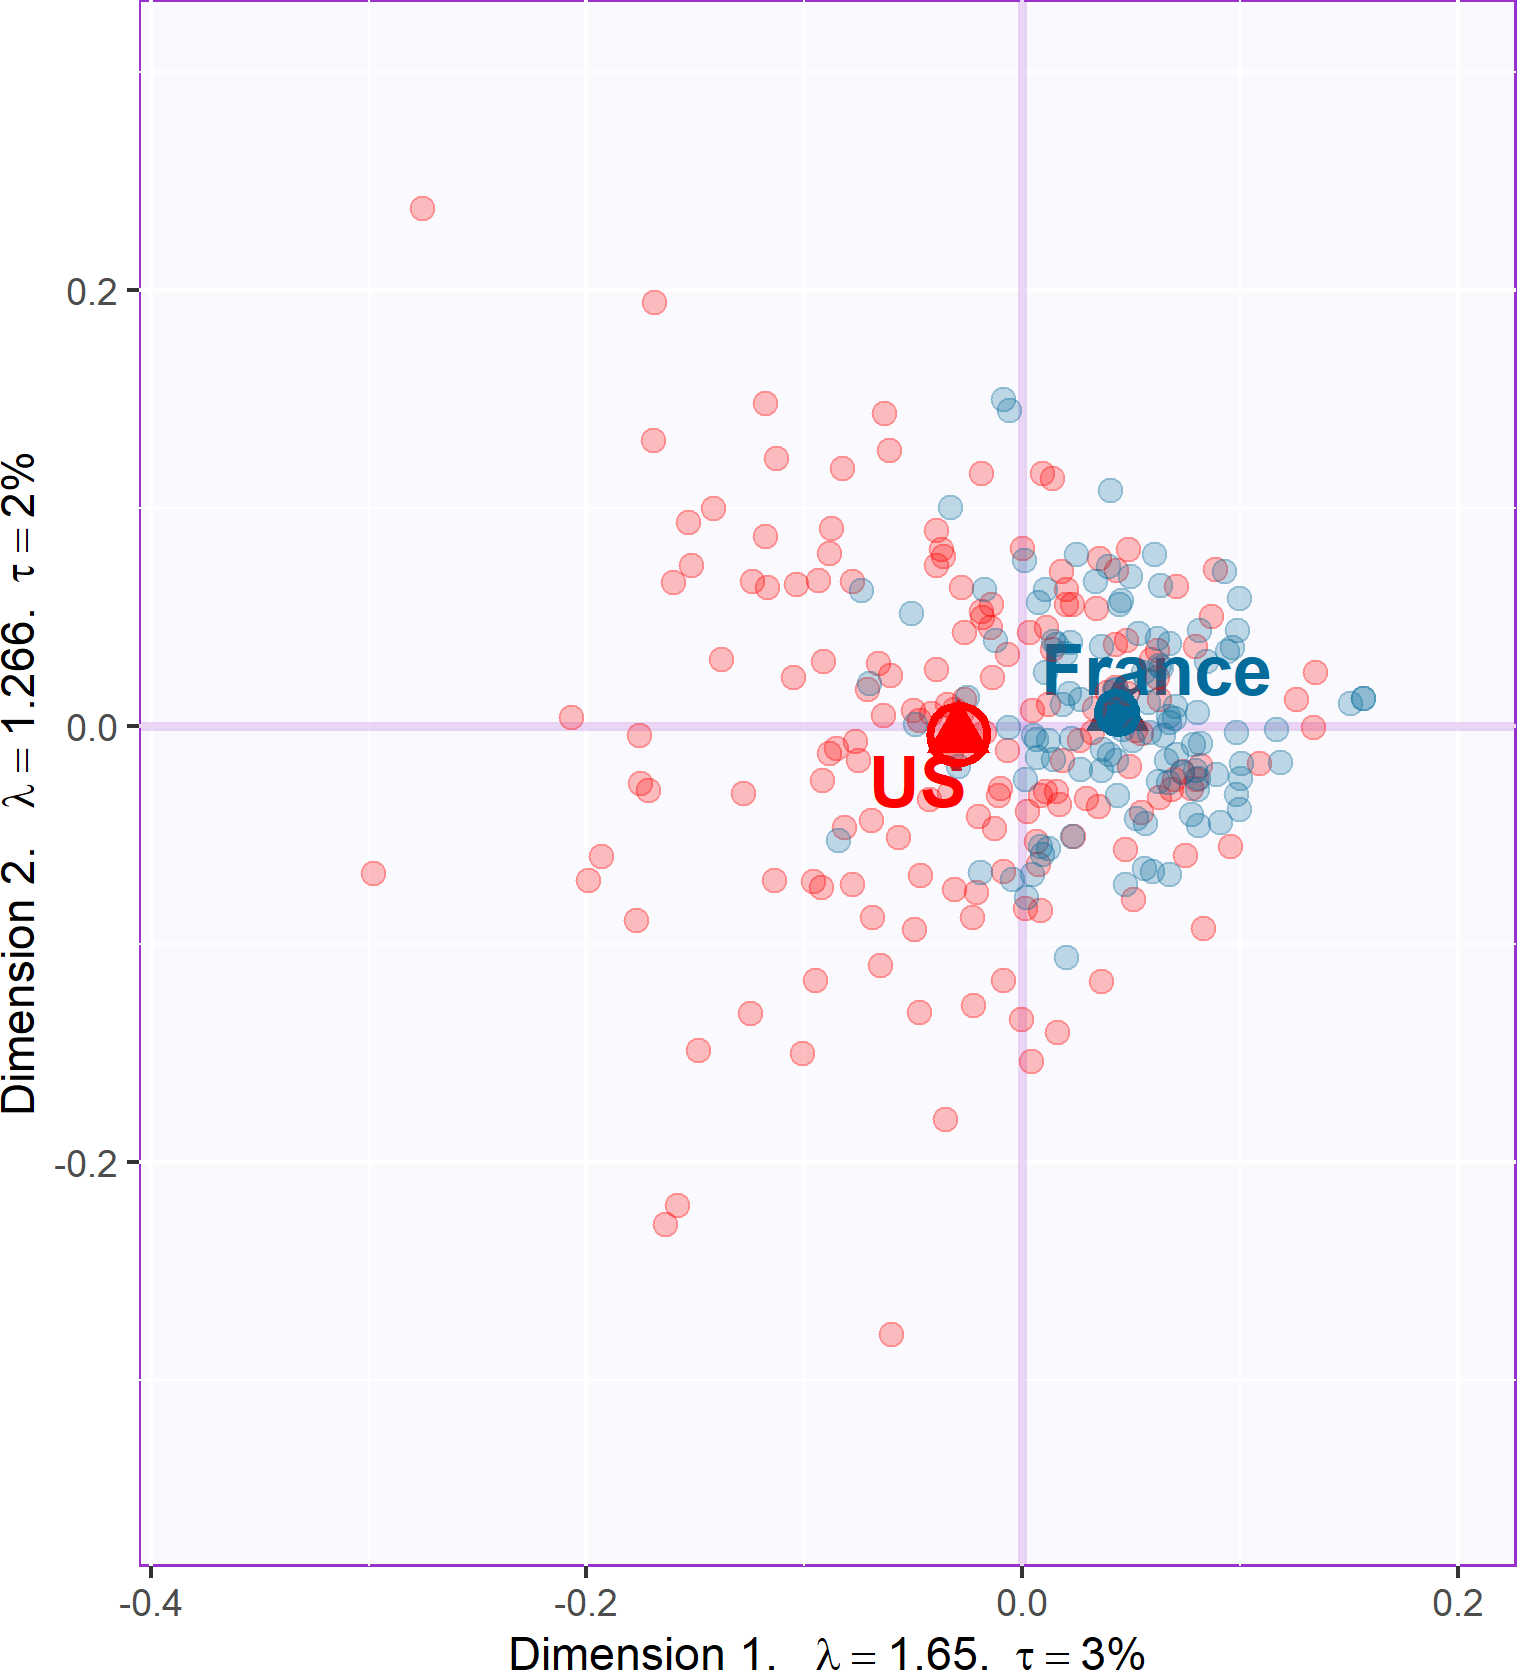
\includegraphics[width=0.4\columnwidth]{./Music-Descriptor-Space_files/figure-latex/map4RVAcode-1.png}
  \label{fig:map4RVA}
  \caption*{\footnotesize \textit{Note.} Axis labels indicate dimension, eigenvalue, and explained variance for that dimension.}
\end{figure}

Figure \ref{fig:map4RVA} displays the factor scores obtained from the MDS performed on the co-occurrence matrix for the AS, along with group means and bootstrap-derived confidence intervals. The separation between the confidence intervals indicates significant differences between French and American participants, \(\textit{p}\). \textless{} .01. Additional analyses using gender identity and level of music training as factors did not reach significance.

\hypertarget{mfa}{%
\paragraph{MFA}\label{mfa}}

Figure \ref{fig:mfasbs} displays the results of the MFAs as partial factor score plots (see ``Multiple Factor Analysis'' above) highlighting differences in descriptions from the perspective of the excerpts (left) and the adjectives (right) between French and American participants. The two separate MFAs revealed slightly different factorial dimensions, as shown by the percentage of extracted variance on each axis (tau), but the general space for both plots is similar to the space revealed by the CA for Experiment 2 (Figure \ref{fig:factormapsA}). Thus we can interpret the space similarly, relative to the valence-arousal plane. However, in this case, we cannot compare elements between maps.

The diamonds represent the compromise between the mental spaces of the French and American participants for each item, and the lines extending from the diamonds to the circles point to the partial factor scores for the items from the perspective of each group (Abdi et al., 2013). Excerpts and adjectives that were rated similarly by each group have short lines extending from them, and those that were rated differently by each group have longer lines. Examples of excerpts that were rated differently are numbers 6, 8, and 12. Adjectives that were used differently include ``Disturbing,'' ``Round,'' ``Solemn,'' and ``Bright.''

\begin{figure}   
  \centering  
  \caption{Compromise (diamonds) and partial factor scores (small circles) for MFA analyses on the Excerpts and Adjectives, colored according to clusters identified by the respective HCAs.}
    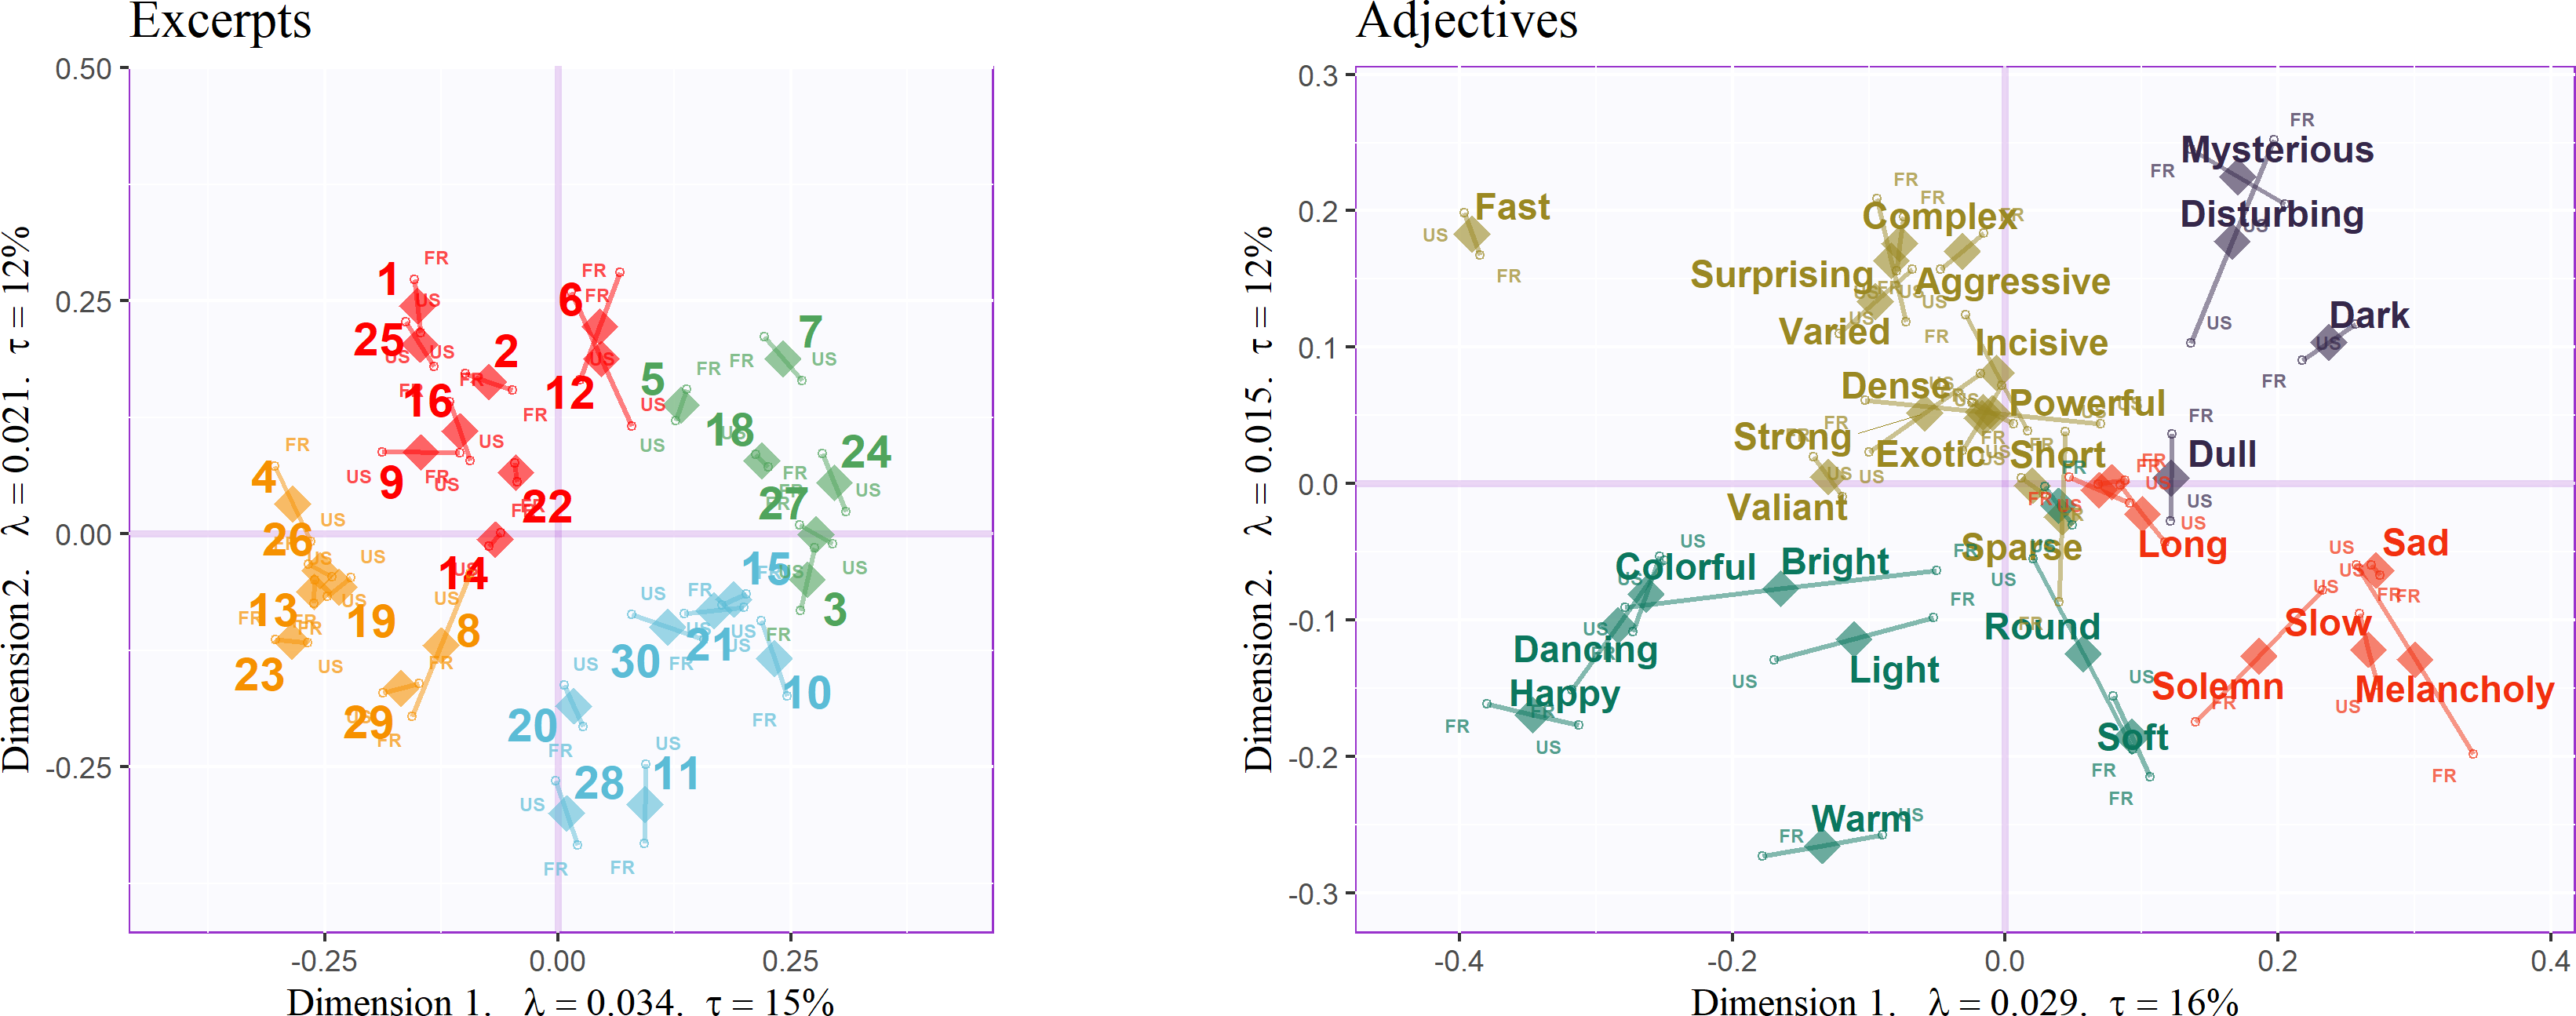
\includegraphics{./Music-Descriptor-Space_files/figure-latex/mfatogether-1.png}
  \label{fig:mfasbs}
  \caption*{\footnotesize \textit{Note.} Axis labels include dimension, eigenvalue, and explained variance for that dimension.}
\end{figure}

\hypertarget{experiment-2-discussion}{%
\subsection{Experiment 2 Discussion}\label{experiment-2-discussion}}

As suggested by the MDS on the participants (Figure \ref{fig:map4RVA}), American and French participants differed in both their mean and their variance. The larger variance of the American participants likely shows that American participants constitute a more heterogeneous group than French participants. This heterogeneity of the American participants is reflected in their varied responses to the nationality question (with nine different answers), compared to the French participants who all responded ``French'' (except for one participant who responded with ``French - Belgian'').

Because participants only rated half of the excerpts, the mean group differences and confidence intervals are meaningful, but the proximity between individual participants can not be directly interpreted as similarity. A better estimation of between-subject similarity would need to weight the similarity (i.e., the number of common adjectives chosen) between two participants by the number of common excerpts presented.\footnote{The results of the CA, on the other hand, are not affected by the fact that participants only rated half of the excerpts.}

The adjectives used in Experiment 2 were selected to engage a cognitive appraisal, but the first two factorial dimensions of the MFA reveal that participants were answering using emotional dimensions such as valence and arousal---a result that resonates with previous work investigating conceptual organization (Osgood \& Suci, 1955) and music and emotion (Wedin, 1969, 1972).

As a consequence, differences between French participants include a large proportion of evaluative adjectives such as ``Bright,'' ``Light,'' ``Round,'' ``Solemn,'' ``Melancholy,'' and ``Disturbing.'' ``Bright'' (Brillant) may be the most extreme example of this intercultural difference, as the French partial factor score is close to the origin and the American partial factor score is further away, a difference suggesting that this word has a more positive valence in English than in French. Additionally, the location of the American partial factor score for ``Bright'' suggests that Americans commonly grouped it with ``Colorful'' (Coloré) and ``Dancing'' (Dansant), a contrast to how the French participants used it. ``Light'' (Clair) shows a similar effect to that of ``Bright'' with respect to the magnitude of difference. The inverse of ``Bright'' and ``Light'' might be ``Round,'' (Tendre), whose French partial factor score is further from the origin than the American. ``Melancholy'' (Mélancolique) and ``Sad'' (Triste) were almost synonymous in English, but not in French. The location of ``Solemn'' (Solennel) suggests that it carries more valence in English, but more arousal in French. ``Disturbing'' (inquiétant) is far from the origin for French participants but not for American participants. All of these differences highlight possible differences in semantic associations and frequency of use between languages.

\hypertarget{experiment-3-combined-surveys}{%
\section{Experiment 3: Combined Surveys}\label{experiment-3-combined-surveys}}

\hypertarget{methods-2}{%
\subsection{Methods}\label{methods-2}}

Because Experiment 3 used the data tables computed for Experiments 1 and 2 for its analysis---Partial Least Squares Correlation (PLSC)---no additional data collection was necessary. However, because PLSC requires the same sets of observations, and because Experiments 1 and 2 removed different excerpts, we removed from the data the excerpts present in only one table. Specifically, Excerpt 17 was removed from the table used in Experiment 1 and Excerpts 6 and 14 were removed from the table used in Experiment 2. This way, both data tables comprised data from the same 27 Excerpts.

\hypertarget{results-2}{%
\subsection{Results}\label{results-2}}

\begin{wrapfigure}{h}{.4\textwidth}  
  \begin{center}
  \caption{PLSC: Scree plot showing explained variance per dimension.}
    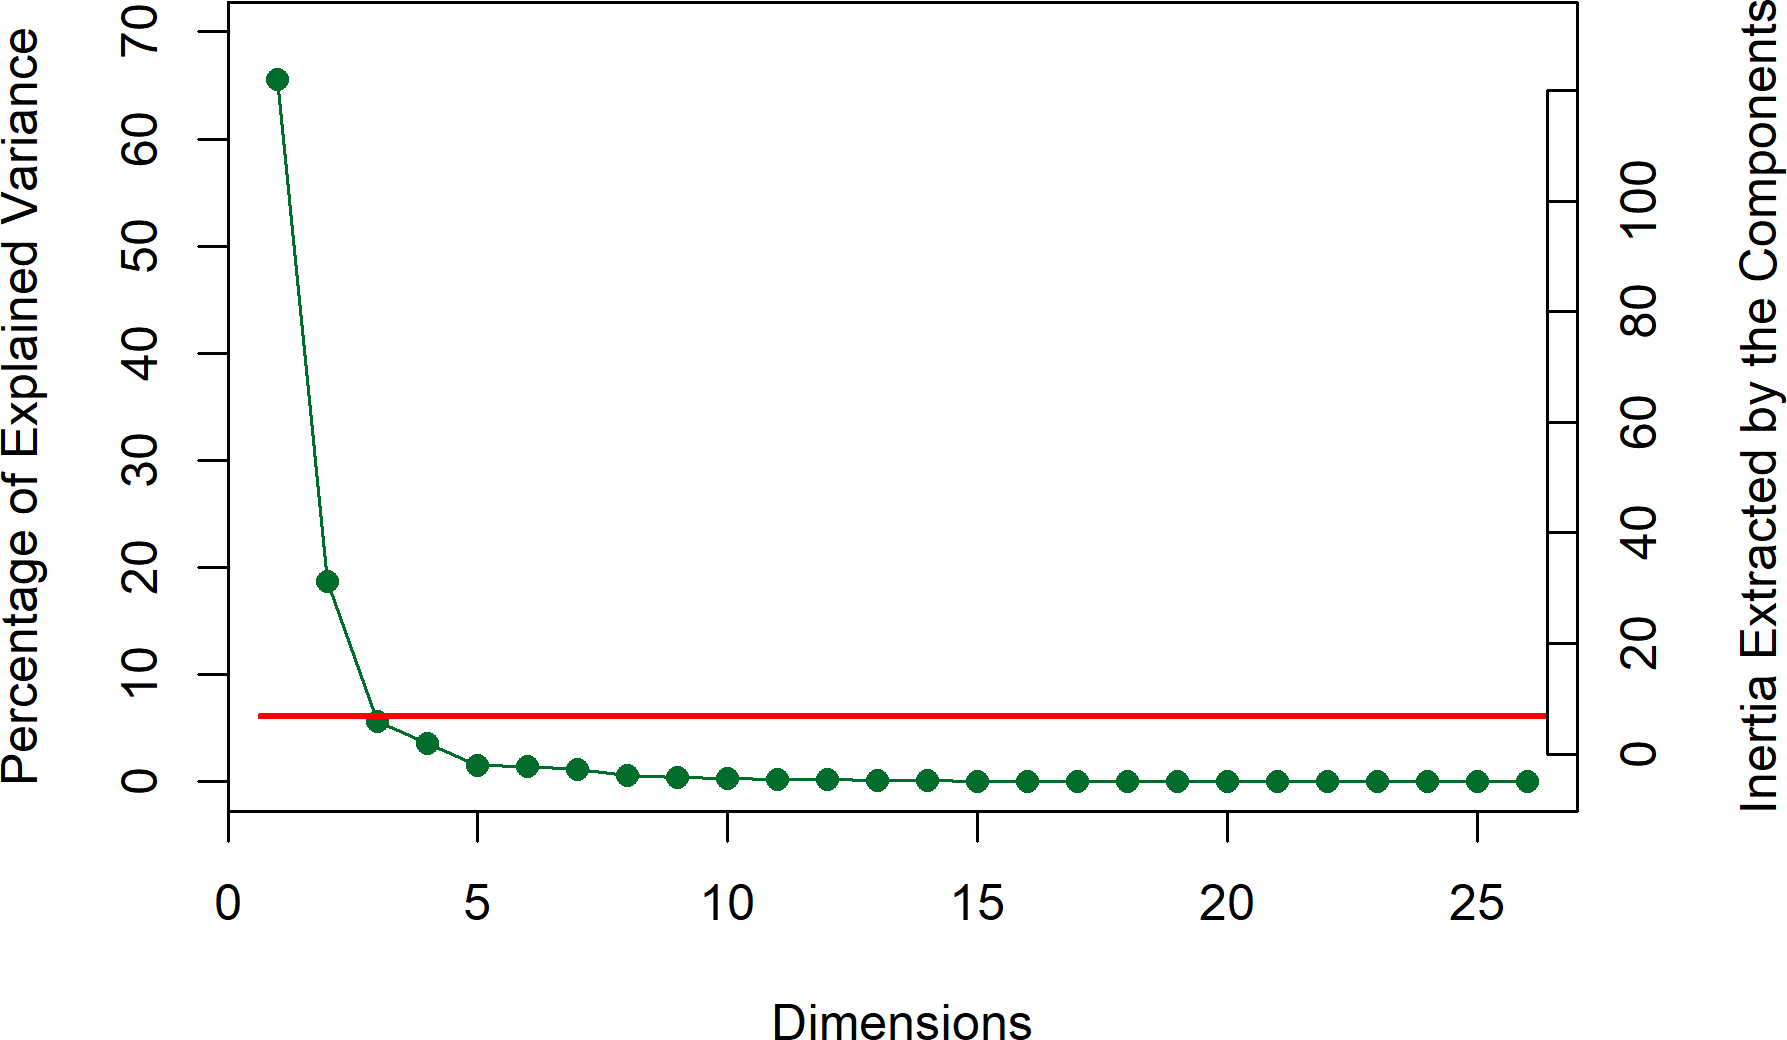
\includegraphics{./Music-Descriptor-Space_files/figure-latex/screePLSCcode-1.png}
  \caption*{Horizontal line represents the average variance extracted per dimension.}\label{fig:screePLSC}  
 \end{center}
\end{wrapfigure}

The PLSC performed using the pseudo-contingency tables from Experiments 1 and 2 revealed two significant dimensions which together accounted for 84.25\% of the total variance.

PLSC displays the latent variable scores of one table against its equivalent for the other table (e.g., LV1 from Table 1 versus LV1 for Table 2). Figure \ref{fig:factorplotsPLSC} displays the LVs plot for LVs 1 and 2. In these plots, the excerpts are ccolored according to the clusters identified by the HCA for Experiment 2, along with tolerance intervals comprising the elements from each cluster. The first LVs (Figure \ref{fig:factorplotsPLSC}, left) separate the excerpts with positive valence and low arousal (gold) from those with negative valence and high arousal (green). The second LVs (Figure \ref{fig:factorplotsPLSC}, right) separate the groups with positive valence and high arousal (red) from excerpts with negative valence and low arousal (blue).

\begin{figure}   
  \centering  
  \caption{PLSC: Latent variables for Experiment 1 contingency table (horizontal, $x$) plotted against latent variables for Experiment 2 contingency table (vertical, $y$), including tolerance intervals, colored according to the groups revealed by Experiment 2.}
  \label{fig:factorplotsPLSC}
    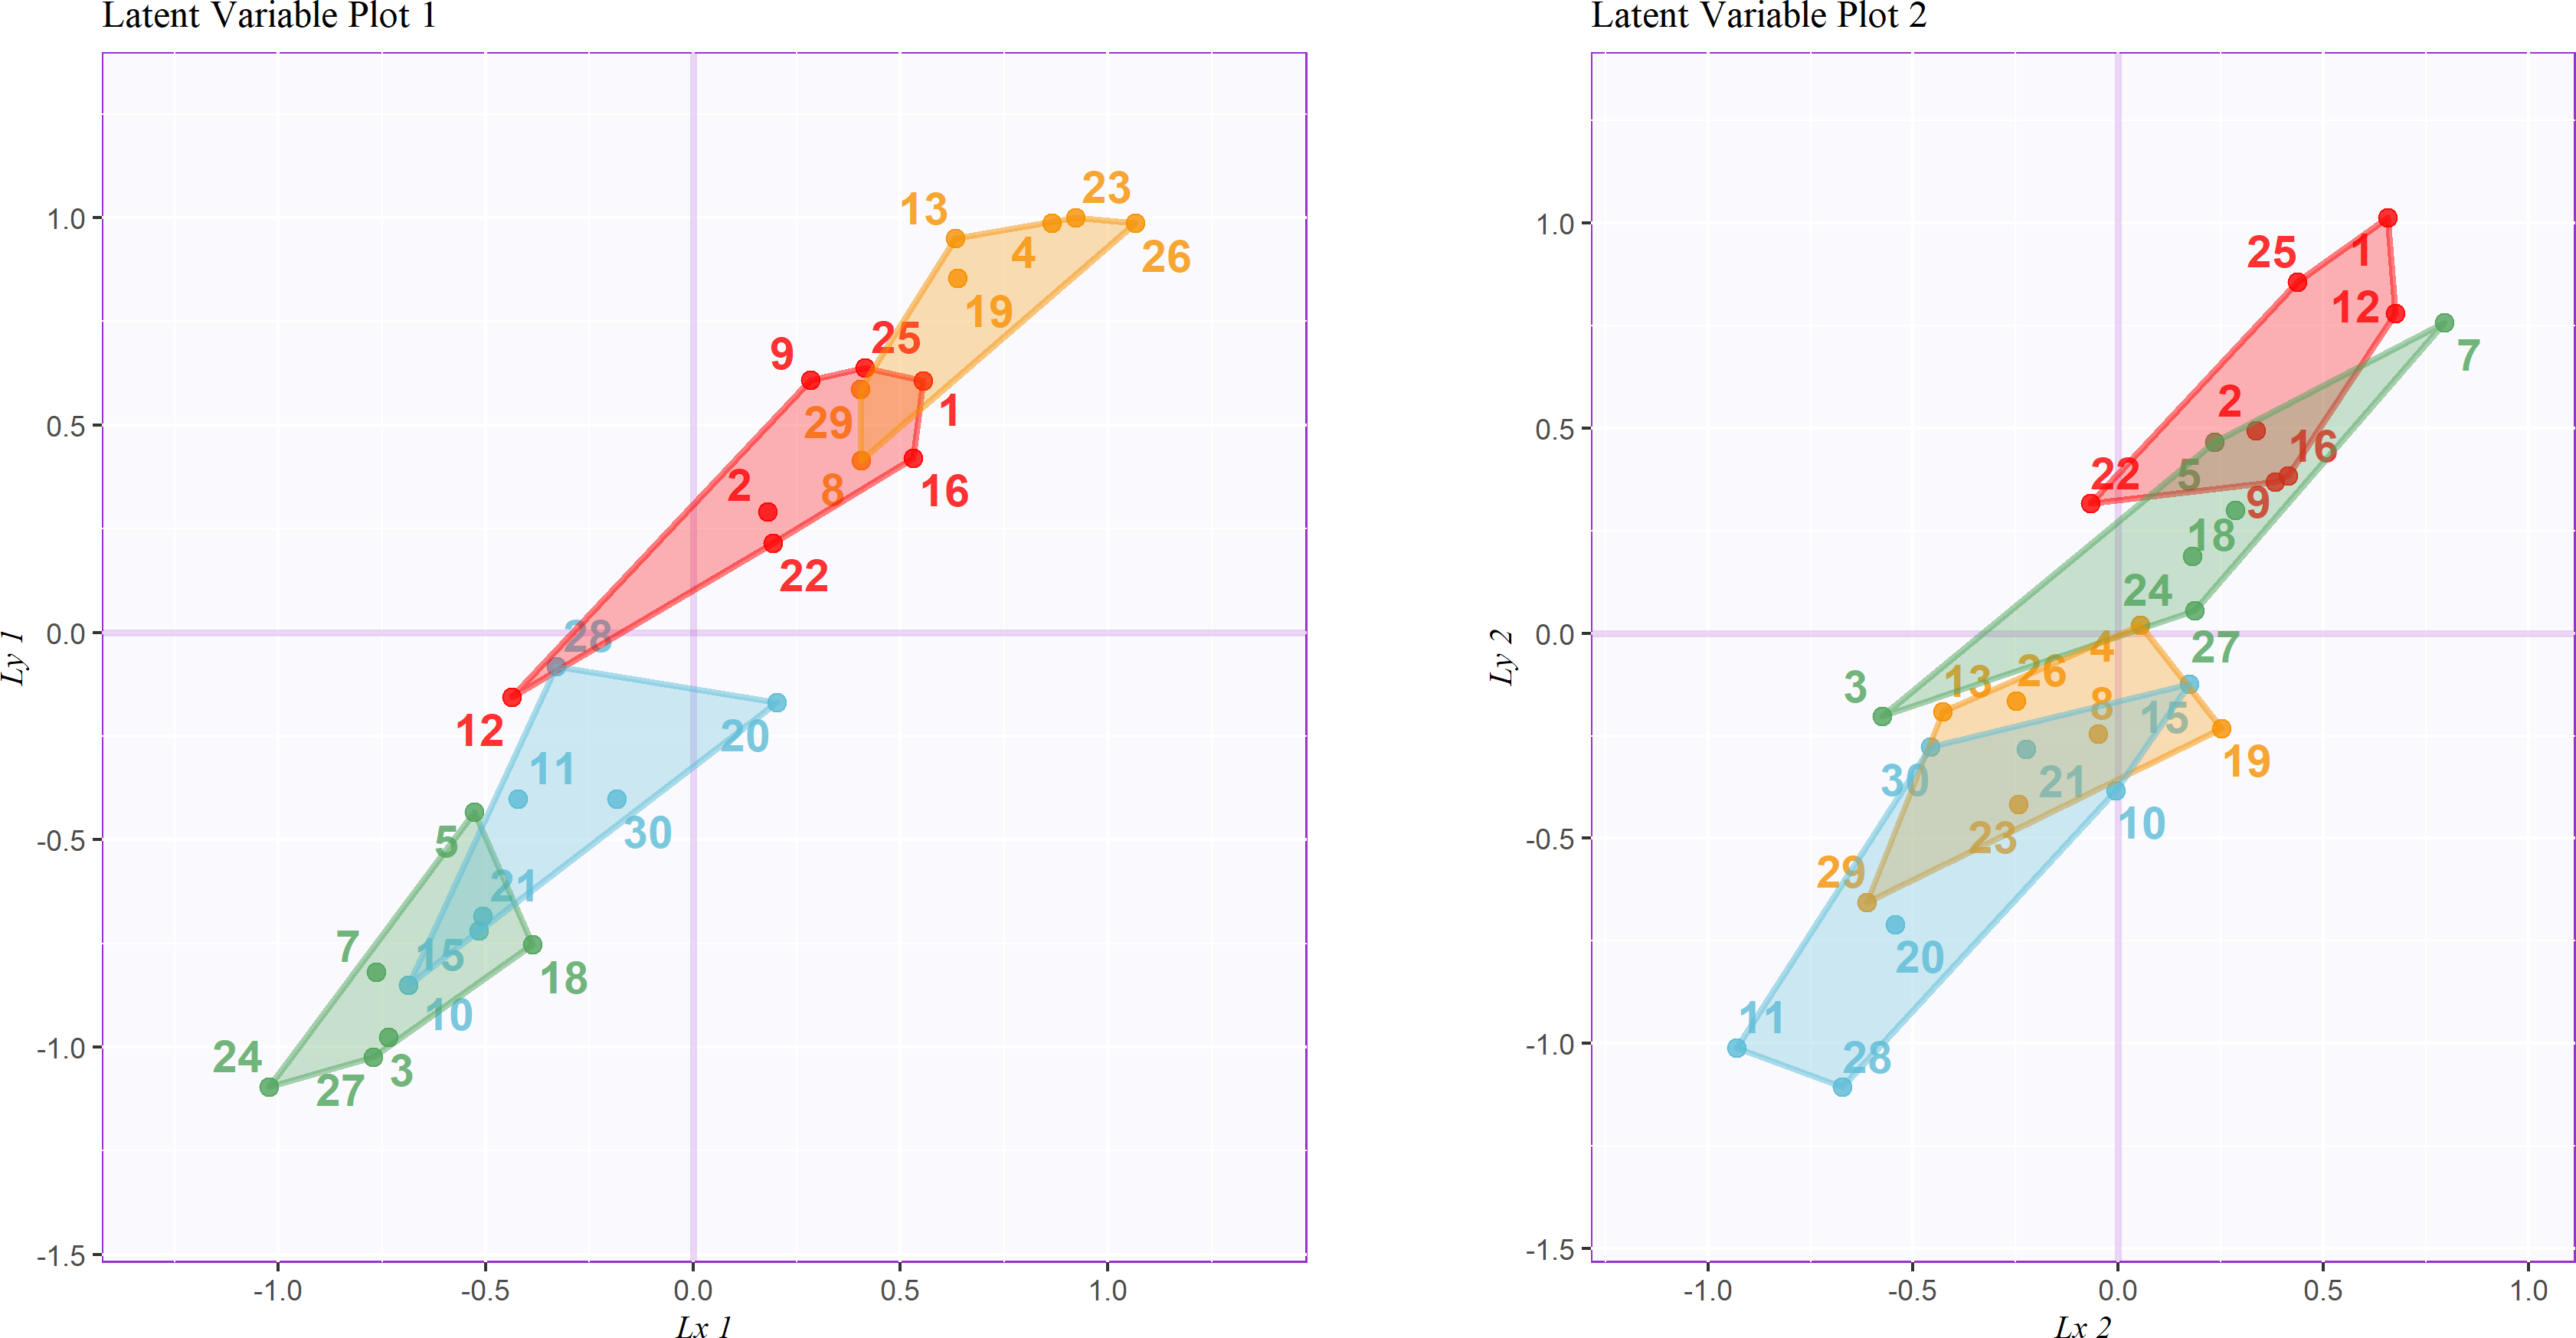
\includegraphics{./Music-Descriptor-Space_files/figure-latex/factorplotsPLSCcode-1.png}
  \caption*{}
\end{figure}

Figure \ref{fig:contsplsc} displays the contributions from the variables from each data table that are important for the first and second LVs. For these plots, the important levels of variables from Experiment 1 are displayed in and green and the important adjectives from Experiment 2 are in blue. The first LVs from each table feature contributions from levels of variables identified as contributing to an arousal dimension in Experiment 1 and the adjectives identified as contributing to a valence dimension in Experiment 2. The second LVs from each table feature contributions from levels of variables identified as contributing to the genre or complexity dimension from Experiment 1 and adjectives identified as contributing to an arousal dimension in Experiment 2.

\begin{figure}   
  \centering  
  \caption{PLSC: Signed contributions important for the first and second latent variables, colored by survey of origin.}
    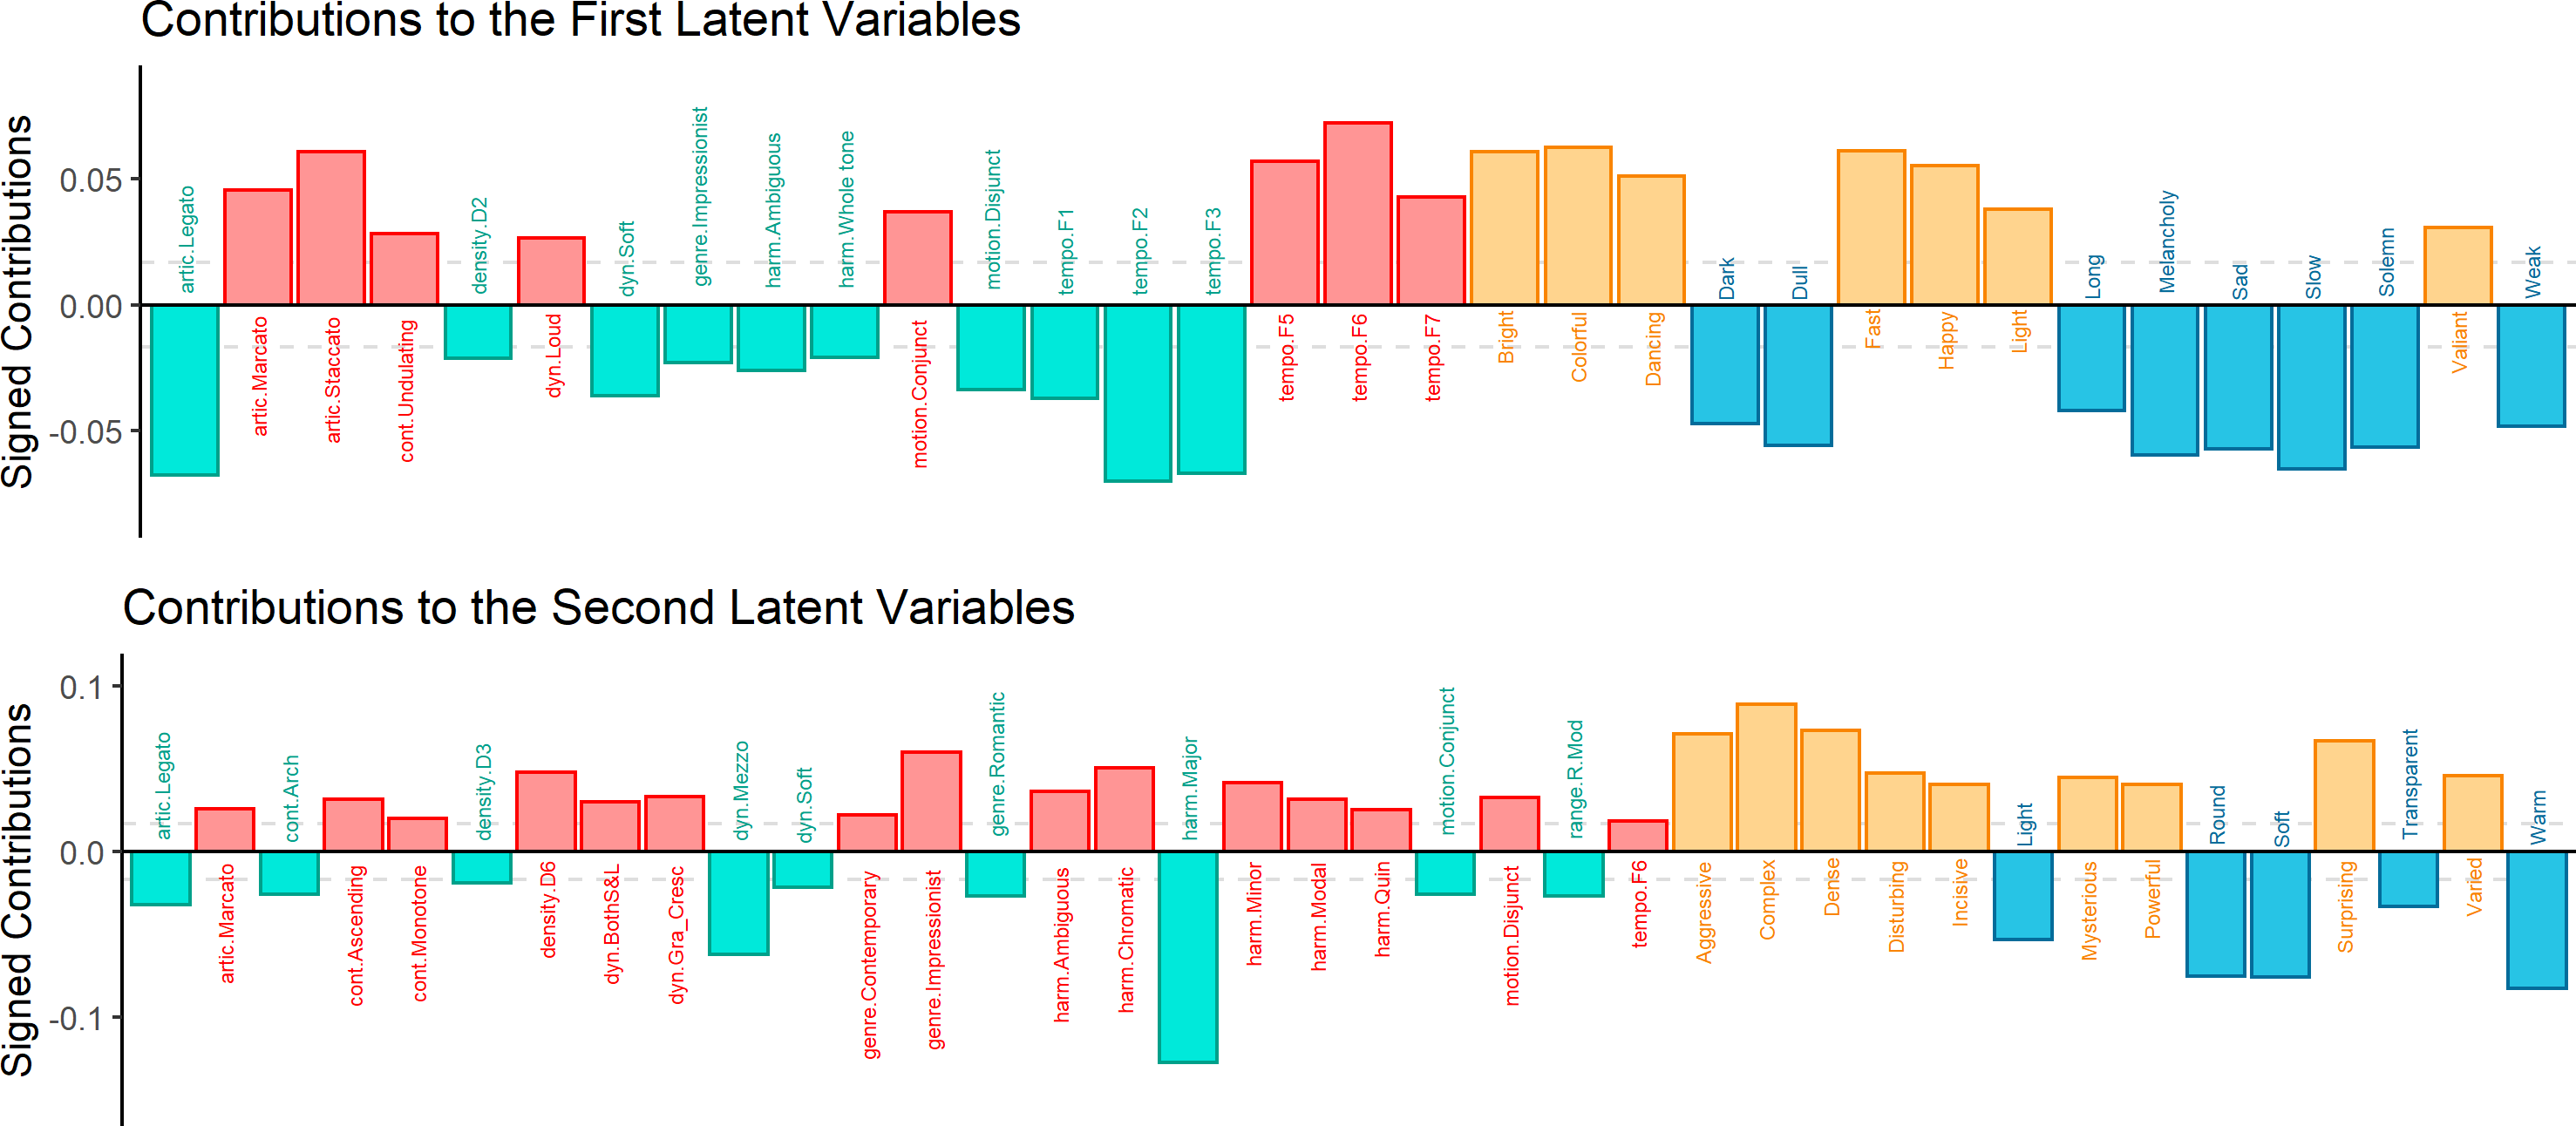
\includegraphics{./Music-Descriptor-Space_files/figure-latex/contsplsccode-1.png}
  \label{fig:contsplsc}
  \caption*{}
\end{figure}

\hypertarget{experiment-3-discussion}{%
\subsection{Experiment 3: Discussion}\label{experiment-3-discussion}}

The goal of this experiment was to identify the common information in the data tables used in Experiments 1 and 2. The first and second latent variables separated the excerpts along dimensions similar to the dimensions extracted by Experiments 1 and 2. Specifically, the first LVs combined the arousal dimension from Experiment 1 with the valence dimension from Experiment 2, and the second LVs combined the complexity or genre dimension from Experiment 1 with the arousal dimension from Experiment 2.

\hypertarget{general-discussion}{%
\section{General Discussion}\label{general-discussion}}

We collected survey responses to musical stimuli and used multivariate analyses to explore the musical and cognitive spaces created by participants from France and the United States. The results revealed commonalities and differences between the two national groups. French and American participants agreed on 1) a clear valence-arousal plane common to participants from both countries when describing the stimuli using adjectives, and 2) a space defined by arousal and complexity when evaluating stimuli using musical qualities. However, French and American participants disagreed on the way in which they used the adjectives when describing the stimuli, a result that suggests either cultural differences in the affective response to the stimuli or, more likely, differences in the use of the adjectives between the two languages.

The results of the MDS analyses across experiments showed group differences between French and American participants when they described excerpts using adjectives (Experiment 2), but these results did not show group differences when experts rated excerpts on specific musical qualities (Experiment 1). This pattern of results suggests that Experiment 1 reveals more about the excerpts themselves rather than about the behavior of participants.

Experiment 3 integrates the results of Experiments 1 and 2, because the first and second latent variables of Experiment 3 essentially combine the dimensions of Experiments 1 and 2. For example, Excerpt 26---a very distal point in the first LV plot in Figure \ref{fig:factorplotsPLSC}---is an important contributor to the first dimensions of the CAs for both Experiments 1 and 2 (see Figures \ref{fig:contributionsQ} and \ref{fig:contributionsA} for the contributions), but is not an important contributor to the second dimensions of Experiments 1 and 2, and is therefore close to the origin in the second LV plot. By contrast, Excerpt 7---a large contributor to to the first and second dimensions of the CAs of both Experiments 1 and 2---is far from the origin in both plots in Figure \ref{fig:factorplotsPLSC}.

The differences in results between Experiments 1 and 2---specifically with regard to Excerpts 6 and 14---demonstrate how small differences in experimental paradigm can provide large differences in perspective. In Experiment 1 (by contrast with Experiment 2), the experts rating the excerpts on specific musical qualities isolated two Excerpts: 6---a minimalist, ostinato based excerpt---and 14---a jazzy excerpt, each the only representative of their style. There are a few possible reasons for this pattern of results, including differences 1) in participant characteristics---experts in Experiment 1 versus non-experts in Experiment 2, and 2) in the way the way the questions in each survey assessed the excerpts---with specific musical qualities in Experiment 1 and subjective evaluations in Experiment 2. Of these two, the second is more likely, because the few participants in Experiment 2 with significant musical training did not differ in their descriptions of the excerpts from the untrained participants.

The different experimental paradigms in the present study all provide useful perspectives. For example, the paradigm from Experiment 1---which separates stimuli along concrete musical dimensions---effectively reveals stimulus differences, whereas the paradigm from Experiment 2 reveals stimulus cognitive and affective similarity. In addition, the combination of these two paradigms (as in Experiment 3) probes the ``why'' of the stimulus affective impact.

\hypertarget{limitations-future-directions}{%
\subsection{Limitations \& future directions}\label{limitations-future-directions}}

Although we evaluated scores and ratings of participants from different countries, we do not explicitly address multiculturality, because France and the United States are both Western countries that share the same Western musical culture. To address this question, an experiment would need to include music and/or participants from multiple, contrasting musical cultures. However, specific musical qualities, such as harmony, may not apply or translate well to other musical cultures, because the concepts of melodic and harmonic material are not the same across all musical cultures (Cohn et al., 2001; Raman \& Dowling, 2017). We also suggest that data collected in this way have a much greater hypothetical reach, but the data collected for these experiments represent a convenience sample, and many of the participants were students. However, this limitation could be easily remedied in future studies.\\
One question that fell beyond the scope of this study was to pinpoint the source of the semantic differences between languages (i.e., ``Bright,'' ``Light,'' ``Round,'' ``Solemn,'' ``Melancholy,'' and ``Disturbing''), illustrated in Figure \ref{fig:mfasbs}. These differences may not reflect true cultural influence of music listening or preference, but simply linguistic differences, including the adjectives' frequency of use in either language or the cultural associations of the words (B. Thompson et al., 2020). Diving more into these questions would be, of course, a fascinating future study.

\hypertarget{conclusions}{%
\section{Conclusions}\label{conclusions}}

On-line data collection and multivariate analysis are not simply a palliative to be used in a time of pandemic. In fact, this paradigm not only enriches the psychologist's methodological tool-box, but it also may be one of the best ways of reaching a more representative population than first year undergraduate students in psychology.

\newpage

\hypertarget{references}{%
\section{References}\label{references}}

\begingroup
\setlength{\parindent}{-0.5in}
\setlength{\leftskip}{0.5in}

\hypertarget{refs}{}
\begin{CSLReferences}{1}{0}
\leavevmode\hypertarget{ref-Abdi2010d}{}%
Abdi, H., \& Williams, L. J. (2010). {Correspondence Analysis}. In N. Salkind (Ed.), \emph{Encyclopedia of research design}. Sage.

\leavevmode\hypertarget{ref-Abdi2013a}{}%
Abdi, H., \& Williams, L. J. (2013). {Partial Least Squares Methods: Partial Least Squares Correlation and Partial Least Square Regression}. In B. Reisfeld \& A. N. Mayeno (Eds.), \emph{Methods in molecular biology: Computational toxicology volume II} (Vol. 930, pp. 549--579). Springer Science+Business Media, LLC. \url{https://doi.org/10.1007/978-1-62703-059-5}

\leavevmode\hypertarget{ref-Abdi2013}{}%
Abdi, H., Williams, L. J., \& Valentin, D. (2013). {Multiple factor analysis: Principal component analysis for multitable and multiblock data sets}. \emph{Wiley Interdisciplinary Reviews: Computational Statistics}, \emph{5}, 149--179. \url{https://doi.org/10.1002/wics.1246}

\leavevmode\hypertarget{ref-Ares2010}{}%
Ares, G., Deliza, R., Barreiro, C., Giménez, A., \& Gámbaro, A. (2010). {Comparison of two sensory profiling techniques based on consumer perception}. \emph{Food Quality and Preference}, \emph{21}(4), 417--426. \url{https://doi.org/10.1016/j.foodqual.2009.10.006}

\leavevmode\hypertarget{ref-Balkwill1999}{}%
Balkwill, L. L., \& Thompson, W. F. (1999). {A Cross-Cultural Investigation of the Perception of Emotion in Music : Psychophysical and Cultural Cues}. \emph{Music Perception: An Interdisciplinary Journal}, \emph{17}(1), 43--64. \url{https://doi.org/10.2307/40285811}

\leavevmode\hypertarget{ref-Balkwill2004}{}%
Balkwill, L. L., Thompson, W. F., \& Matsunaga, R. (2004). {Recognition of emotion in Japanese, Western, and Hindustani music by Japanese listeners}. \emph{Japanese Psychological Research}, \emph{46}(4), 337--349. \url{https://doi.org/10.1111/j.1468-5584.2004.00265.x}

\leavevmode\hypertarget{ref-Bartlett1980a}{}%
Bartlett, J. C., \& Dowling, W. J. (1980). {Recognition of transposed melodies: A key-distance effect in developmental perspective}. \emph{Journal of Experimental Psychology: Human Perception and Performance}, \emph{6}(3), 501--515. \url{https://doi.org/10.1037/0096-1523.6.3.501}

\leavevmode\hypertarget{ref-Battcock2019}{}%
Battcock, A., \& Schutz, M. (2019). {Acoustically expressing affect}. \emph{Music Perception}, \emph{37}(1), 66--91. \url{https://doi.org/10.1525/MP.2019.37.1.66}

\leavevmode\hypertarget{ref-Benzecri1973}{}%
Benzécri, J.-P. (1973). \emph{{L'analyse des données.}} Dunod.

\leavevmode\hypertarget{ref-Bigand2006}{}%
Bigand, E., \& Poulin-Charronnat, B. (2006). {Are we "experienced listeners"? A review of the musical capacities that do not depend on formal musical training}. \emph{Cognition}, \emph{100}(1), 100--130. \url{https://doi.org/10.1016/j.cognition.2005.11.007}

\leavevmode\hypertarget{ref-Bigand2005}{}%
Bigand, E., Vieillard, S., Madurell, F., Marozeau, J., \& Dacquet, A. (2005). {Multidimensional scaling of emotional responses to music: The effect of musical expertise and of the duration of the excerpts}. \emph{Cognition and Emotion}, \emph{19}(8), 1113--1139. \url{https://doi.org/10.1080/02699930500204250}

\leavevmode\hypertarget{ref-Borg2005}{}%
Borg, I., \& Groenen, P. J. F. (2005). \emph{{Modern Multidimensional Scaling}} (2nd ed., Vol. 36). Springer Science+Business Media, Inc.

\leavevmode\hypertarget{ref-BrunerII1990}{}%
Bruner II, G. C. (1990). {Music, Mood, and Marketing}. \emph{Journal of Marketing}, \emph{October}, 94--104.

\leavevmode\hypertarget{ref-Cohn2001}{}%
Cohn, R., Hyer, B., Dahlhaus, C., Anderson, J., \& Wilson, C. (2001). \emph{{Harmony}}. Oxford University Press.

\leavevmode\hypertarget{ref-Coombs1956}{}%
Coombs, C. H., Milholland, J. E., \& Womer, F. B. (1956). {The assessment of partial knowledge}. \emph{Educational and Psychological Measurement}, \emph{16}(1), 13--37. \url{https://doi.org/10.1177/001316445601600102}

\leavevmode\hypertarget{ref-Cowen2020}{}%
Cowen, A. S., Fang, X., Sauter, D., \& Keltner, D. (2020). {What music makes us feel: At least 13 dimensions organize subjective experiences associated with music across different cultures}. \emph{Proceedings of the National Academy of Sciences of the United States of America}, \emph{117}(4), 1924--1934. \url{https://doi.org/10.1073/pnas.1910704117}

\leavevmode\hypertarget{ref-Darrow1987}{}%
Darrow, A. A., Haack, P., \& Kuribayashi, F. (1987). {Descriptors and Preferences for Eastern and Western Musics by Japanese and American Nonmusic Majors}. \emph{Journal of Research in Music Education}, \emph{35}(4), 237--248. \url{https://doi.org/10.2307/3345076}

\leavevmode\hypertarget{ref-Dowling1978a}{}%
Dowling, W. J. (1978). {Scale and Contour: Two Components of a Theory of Memory for Melodies}. \emph{Psychological Review}, \emph{85}(4), 341--354. \url{https://doi.org/10.1037/0033-295X.85.4.341}

\leavevmode\hypertarget{ref-Escofier1994}{}%
Escofier, B., \& Pagès, J. (1994). {Multiple factor analysis (AFMULT package)}. \emph{Computational Statistics and Data Analysis}, \emph{18}(1), 121--140. \url{https://doi.org/10.1016/0167-9473(94)90135-X}

\leavevmode\hypertarget{ref-Escofier-Cordier1965}{}%
Escofier-Cordier, B. (1965). \emph{{L'analyse des correspondances}} {[}Doctoral Thesis{]}. Universit{é} de Rennes.

\leavevmode\hypertarget{ref-Fritz2009}{}%
Fritz, T., Jentschke, S., Gosselin, N., Sammler, D., Peretz, I., Turner, R., Friederici, A. D., \& Koelsch, S. (2009). {Universal Recognition of Three Basic Emotions in Music}. \emph{Current Biology}, \emph{19}(7), 573--576. \url{https://doi.org/10.1016/j.cub.2009.02.058}

\leavevmode\hypertarget{ref-Gray1967}{}%
Gray, P. H., \& Wheeler, G. E. (1967). {The Semantic Differential as an Instrument to Examine the Recent Folksong Movement}. \emph{Journal of Social Psychology}, \emph{72}(2), 241--247. \url{https://doi.org/10.1080/00224545.1967.9922321}

\leavevmode\hypertarget{ref-Greenacre1984}{}%
Greenacre, M. J. (1984). \emph{{Theory and Applications of Correspondence Analysis}}. Academic Press.

\leavevmode\hypertarget{ref-Gregory1996}{}%
Gregory, A. H., \& Varney, N. (1996). {Cross-cultural comparisons in the affective response to music}. \emph{Psychology of Music}, \emph{24}(1), 47--52. \url{https://doi.org/10.1177/0305735696241005}

\leavevmode\hypertarget{ref-Hesterberg2011}{}%
Hesterberg, T. (2011). {Bootstrap}. \emph{Wiley Interdisciplinary Reviews: Computational Statistics}, \emph{3}(6), 497--526. \url{https://doi.org/10.1002/wics.182}

\leavevmode\hypertarget{ref-Juslin2010}{}%
Juslin, P. N., \& Sloboda, J. A. (Eds.). (2010). \emph{{Handbook of music and emotion: Theory, research, applications.}} Oxford University Press.

\leavevmode\hypertarget{ref-Juslin2008a}{}%
Juslin, P. N., \& Västfjäll, D. (2008). {All emotions are not created equal: Reaching beyond the traditional disputes}. \emph{Behavioral and Brain Sciences}, \emph{31}, 559--621. \url{https://doi.org/doi:10.1017/S0140525X08005554\%20Patrik}

\leavevmode\hypertarget{ref-Katz1933}{}%
Katz, D., \& Braly, K. (1933). {Racial stereotypes of one hundred college students}. \emph{Journal of Abnormal and Social Psychology}, \emph{28}(3), 280--290. \url{https://doi.org/10.1037/h0074049}

\leavevmode\hypertarget{ref-Kopacz2005}{}%
Kopacz, M. (2005). {Personality and music preferences: The influence of personality traits on preferences regarding musical elements}. \emph{Journal of Music Therapy}, \emph{42}(3), 216--239. \url{https://doi.org/10.1093/jmt/42.3.216}

\leavevmode\hypertarget{ref-Krishnan2011}{}%
Krishnan, A., Williams, L. J., McIntosh, A. R., \& Abdi, H. (2011). {Partial Least Squares (PLS) methods for neuroimaging: A tutorial and review}. \emph{NeuroImage}, \emph{56}(2), 455--475. \url{https://doi.org/10.1016/j.neuroimage.2010.07.034}

\leavevmode\hypertarget{ref-Ladinig2012}{}%
Ladinig, O., \& Schellenberg, E. G. (2012). {Liking unfamiliar music: Effects of felt emotion and individual differences}. \emph{Psychology of Aesthetics, Creativity, and the Arts}, \emph{6}(2), 146--154. \url{https://doi.org/10.1037/a0024671}

\leavevmode\hypertarget{ref-Madsen1997}{}%
Madsen, C. K. (1997). {Emotional Response to Music as Measured by the Two-Dimensional CRDI}. \emph{Journal of Music Therapy}, \emph{34}(3), 187--199. \url{https://doi.org/10.1093/jmt/34.3.187}

\leavevmode\hypertarget{ref-Meyners2014}{}%
Meyners, M., \& Castura, J. (2014). {Check-All-That-Apply Questions}. In \emph{Novel techniques in sensory characterization and consumer profiling} (pp. 271--306). CRC Press/Taylor {\&} Francis. \url{https://doi.org/10.1201/b16853-12}

\leavevmode\hypertarget{ref-Osgood1955}{}%
Osgood, C. E., \& Suci, G. J. (1955). {Factor analysis of meaning}. \emph{Journal of Experimental Psychology}, \emph{50}(5), 325--338. \url{https://doi.org/10.1037/h0043965}

\leavevmode\hypertarget{ref-Pielou1984}{}%
Pielou, E. C. (1984). \emph{{The Interpretation of Ecological Data: A Primer on Classification and Ordination}}. Wiley.

\leavevmode\hypertarget{ref-Raman2016}{}%
Raman, R., \& Dowling, W. J. (2016). {Real-Time Probing of Modulations in South Indian Classical (Carnātic) Music by Indian and Western Musicians}. \emph{Music Perception}, \emph{33}(3), 367--393. \url{https://doi.org/10.1525/MP.2016.33.03.367}

\leavevmode\hypertarget{ref-Raman2017}{}%
Raman, R., \& Dowling, W. J. (2017). {Perception of modulations in south indian classical (carnatic) music by student and teacher musicians: A cross-cultural study}. \emph{Music Perception}, \emph{34}(4), 424--437.

\leavevmode\hypertarget{ref-Roda2014}{}%
Rodà, A., Canazza, S., \& De Poli, G. (2014). {Clustering affective qualities of classical music: Beyond the valence-arousal plane}. \emph{IEEE Transactions on Affective Computing}, \emph{5}(4), 364--376. \url{https://doi.org/10.1109/TAFFC.2014.2343222}

\leavevmode\hypertarget{ref-Thompson2020}{}%
Thompson, B., Roberts, S. G., \& Lupyan, G. (2020). {Cultural influences on word meanings revealed through large-scale semantic alignment}. \emph{Nature Human Behaviour}, \emph{4}(10), 1029--1038. \url{https://doi.org/10.1038/s41562-020-0924-8}

\leavevmode\hypertarget{ref-Thompson1994}{}%
Thompson, W. F. (1994). {Sensitivity to combinations of musical parameters: Pitch with duration, and pitch pattern with durational pattern}. \emph{Perception {\&} Psychophysics}, \emph{56}(3), 363--374. \url{https://doi.org/10.3758/BF03209770}

\leavevmode\hypertarget{ref-Tucker1958}{}%
Tucker, L. R. (1958). {An inter-battery method of factor analysis}. \emph{Psychometrika}, \emph{23}(2), 111--136. \url{https://doi.org/10.1007/BF02289009}

\leavevmode\hypertarget{ref-Valentin2012}{}%
Valentin, D., Chollet, S., Lelièvre, M., \& Abdi, H. (2012). {Quick and dirty but still pretty good: a review of new descriptive methods in food science}. \emph{International Journal of Food Science {\&} Technology}, 1--16. \url{https://doi.org/10.1111/j.1365-2621.2012.03022.x}

\leavevmode\hypertarget{ref-Wallmark2019}{}%
Wallmark, Z. (2019). {A corpus analysis of timbre semantics in orchestration treatises}. \emph{Psychology of Music}, \emph{47}(4), 585--605. \url{https://doi.org/10.1177/0305735618768102}

\leavevmode\hypertarget{ref-Wedin1969}{}%
Wedin, L. (1969). {Dimension Analysis of Emotional Expression in Music}. \emph{Swedish Journal of Musicology}, \emph{51}, 119--140.

\leavevmode\hypertarget{ref-Wedin1972}{}%
Wedin, L. (1972). {Evaluation of a Three-Dimensional Model of Emotional Expression in Music}. \emph{The Psychological Laboratories}, \emph{54}(349), 115--131.

\leavevmode\hypertarget{ref-Zacharakis2014}{}%
Zacharakis, A., Pastiadis, K., \& Reiss, J. D. (2014). {An Interlanguage Study of Musical Timbre Semantic Dimensions and Their Acoustic Correlates}. \emph{Music Perception: An Interdisciplinary Journal}, \emph{31}(4), 339--358. \url{https://doi.org/10.1525/MP.2014.31.4.339}

\leavevmode\hypertarget{ref-Zacharakis2015}{}%
Zacharakis, A., Pastiadis, K., \& Reiss, J. D. (2015). {An Interlanguage Unification of Musical Timbre: Bridging Semantic, Perceptual, and Acoustic Dimensions}. \emph{Music Perception: An Interdisciplinary Journal}, \emph{32}(4), 394--412. \url{https://doi.org/10.1525/MP.2015.32.4.394}

\leavevmode\hypertarget{ref-Zampini2004}{}%
Zampini, M., \& Spence, C. (2004). {The role of auditory cues in modulating the perceived crispness and staleness of potato chips}. \emph{Journal of Sensory Studies}, \emph{19}(5), 347--363. \url{https://doi.org/10.1111/j.1745-459x.2004.080403.x}

\end{CSLReferences}

\endgroup


\end{document}
